\documentclass[a4paper,oneside]{book}
\usepackage[utf8]{vietnam}
\usepackage{amsmath}
\usepackage{amsfonts}
\usepackage{amssymb}
\usepackage{graphicx}
\usepackage{subfig} % gói lệnh cho vẽ nhiều hình trong 1 hình
%\usepackage{subcaption} % gói lệnh cho vẽ nhiều hình trong 1 hình
\usepackage{wrapfig} % gói lệnh vẽ chèn hình vào giữa văn bản
\usepackage{array}  % gói lệnh kẻ bảng với kích thước cố định
\usepackage{tabu}
\usepackage{xcolor}
\usepackage{enumerate} % gói lệnh danh sách
\usepackage[unicode]{hyperref} % gói lệnh tạo liên kết
\usepackage{indentfirst} % Thụt vào đầu mỗi đoạn
\usepackage{pageborder}
\usepackage{comment} %comment khoi lenh
\usepackage{fancybox} 
\usepackage{multirow}
\usepackage{multicol}
\usepackage[left=3.5cm,right=2cm,top=2cm,bottom=2cm]{geometry}
\usepackage{scrextend}
\changefontsizes{13pt} % đặt phông chữ kích thước 13
\linespread{1.2}  % line space multiple 1.2
 \usepackage{fancyhdr}
 \pagestyle{fancy}
 \fancyhf{}
 \usepackage{listings} %Dùng cho định dạng khối lệnh
 \lstset{
 	language=c++, %% Troque para PHP, C, Java, etc... bash é o padrão
 	basicstyle=\ttfamily\small,
 	numberstyle=\footnotesize,
 	% numbers=left,
 	backgroundcolor=\color{gray!10},
 	frame=single,
 	tabsize=2,
 	rulecolor=\color{black!30},
 	title=\lstname,
 	escapeinside={\%*}{*)},
 	breaklines=true,
 	breakatwhitespace=true,
 	framextopmargin=2pt,
 	framexbottommargin=2pt,
 	extendedchars=false,
 	showstringspaces=false,
 	inputencoding=utf8}

\lhead{GVHD: TS. Nguyễn Xuân Hạ}
%\rhead{Luận văn Tốt nghiệp Hệ Cao học Cơ điện tử}

%  \fancyhead[RO]{\rightmark}
\cfoot{\thepage}

\author{Nguyễn Văn Huy}


% ============ BEGIN =================================
\begin{document}
\thispagestyle{empty}
\thisfancypage{
	\setlength{\fboxsep}{0pt}
	\fbox}{} 
\begin{center}
	\begin{large}
		TRƯỜNG ĐẠI HỌC BÁCH KHOA HÀ NỘI
	\end{large} \\
	\begin{large}
		VIỆN CƠ KHÍ
	\end{large} \\
	\begin{normalsize}
	BỘ MÔN CƠ SỞ THIẾT KẾ MÁY \& ROBOT
	\end{normalsize} \\
	\textbf{--------------------  *  ---------------------}\\
	
	\begin{figure}[ht]
		\centering
		% \includegraphics[width=0.2\linewidth]{figs/HUST.png}
	\end{figure}
	
	{\fontsize{32pt}{1}\selectfont LUẬN VĂN}\\%[0.1cm]
	{\fontsize{34pt}{1} \textbf{\textrm{TỐT NGHIỆP CAO HỌC}}}\\%[0.2cm]%\selectfont
	{\fontsize{20pt}{1}\selectfont \textbf{NGÀNH CƠ ĐIỆN TỬ}}\\[0.5cm]
	{\fontsize{20pt}{1}\selectfont  \textbf{...} }\\[2cm]
\end{center}

\hspace{3cm}Sinh viên thực hiện:  \hspace{37pt}% 
\textbf{\parbox[t]{5cm}{    
		Nguyễn Văn Huy
}}

\hspace{3cm}Mã số sinh viên:  \hspace{58pt}% 
\textbf{\parbox[t]{5cm}{    
		20131782\\
		Lớp KT CĐT 01 - K58
}}

\hspace{3cm} Giáo viên hướng dẫn: \hspace{21pt} \textbf{\parbox[t]{5cm}{    
		TS. Nguyễn Xuân Hạ
}}

\hspace{3cm} Giáo viên phản biện: \hspace{24pt} \textbf{\parbox[t]{6cm}{    
		ThS. Nguyễn Minh Quân
}}\\[10pt]

\vspace{2.5cm}
\begin{center}
	{\fontsize{16pt}{1}\selectfont HÀ NỘI 1-2018}
\end{center}



%\frontmatter

\setcounter{page}{4} % Đặt vị trí bắt đầu đếm số trang
\newpage

%\newpage
\begin{center}
    LỜI CẢM ƠN
\end{center}

Tôi xin bày tỏ lòng biết ơn chân thành tới Thầy TS. Nguyễn Xuân Hạ, người đã hướng dẫn tận tình và tạo mọi điều kiện tốt nhất cho tôi hoàn thành luận văn này. Đồng thời tôi xin chân thành cảm ơn tới các Thầy, Cô đã giảng dạy và giúp đỡ tôi trong quá trình nghiên cứu học tập Thạc sĩ tại Trường Đại học Bách Khoa Hà Nội. Các Thầy, Cô đã tận tình truyền đạt kiến thức, kinh nghiệm và cảm hứng cho tôi trong quá trình học tập và nghiên cứu cho tới khi hoàn thiện luận văn này.

Bên cạnh đó, tôi xin chân thành cảm ơn tới gia đình, các anh chị bạn bè đồng nghiệp, các em khóa sau đã hỗ trợ tôi trong quá trình nghiên cứu.

Một lần nữa tôi xin chân thành cảm ơn!

\hspace{2cm}

\begin{center}
    TÓM TẮT NỘI DUNG LUẬN VĂN
\end{center}

Trong luận văn này, tác giả tập trung giải quyết hai vấn đề chính: ứng dụng hệ điều hành robot ROS trong điều khiển robot tự hành thông minh và cải tiến hệ thống tránh vật cản bằng cách phối hợp nhiều tầng cảm biến. Dựa vào các tài liệu, mã nguồn mở tác giả nghiên cứu giải thuật điều khiển robot tự hành, trực tiếp trên nền tảng robot tự hành Dashgo D1. Nội dung luận văn đảm bảo tính khoa học về các vấn đề trong điều khiển robot tự hành, có tính thực tiễn cao. Trong tương lai, tác giả sẽ tối ưu, module hóa hệ thống điều khiển và tránh vật cản cho robot để có thể áp dụng trực tiếp vào công nghiệp, vào đời sống.

\hspace{3cm}

\hspace{7cm} \today \\

\hspace{8cm} HỌC VIÊN \\

\hspace{30pt}

\hspace{7.5cm} Nguyễn Văn Huy

%\newpage

Đây là danh mục kí hiệu


\tableofcontents % chèn mục  lục
\addcontentsline{toc}{chapter}{MỤC LỤC}
\listoffigures % chèn danh sách hình 
\addcontentsline{toc}{chapter}{DANH SÁCH HÌNH VẼ}
% \listoftables % chèn danh sách bảng biểu
% \addcontentsline{toc}{chapter}{DANH SÁCH BẢNG}

\mainmatter
\fancyhead[LO]{\leftmark}
\cfoot{}
\rfoot{\thepage}
\lfoot{Học viên: Nguyễn Văn Huy 180009- Lớp CH2018B}
\renewcommand{\headrulewidth}{2pt} % cho header
\renewcommand{\footrulewidth}{2pt} % cho footer

%----Nội dung---------------------------------------
\chapter{Tổng quan nghiên cứu}
\label{chap:1tqnc}
\section{Giới thiệu robot tự hành}

% - Thế nào là robot tự hành thông minh
% - ứng dụng của robot tự hành thông

%%% Tài liệu tham khảo:
% http://ais.informatik.uni-freiburg.de/teaching/ss18/robotics/ Bài Introduction
% 

Trước đây, nghành robotics tập trung vào nghiên cứu và chế tạo cánh tay robot công nghiệp. Nó được coi như là robot truyền thống (\figurename{\ref{fig:RBCongNghiep}}). Bởi vậy khi nói đến thuật ngữ robot người ta thường nghĩ ngay đến cánh tay robot công nghiệp. \figurename{\ref{fig:RBCongNghiep}} là hình ảnh các cánh tay robot đang làm việc trong khâu sơn khung xe oto. Chúng ta không thấy bóng dáng con người ở trong bức hình này, bởi vì robot công nghiệp truyền thống phải làm việc trong không gian cách ly với con người, có hàng rào bảo vệ vì các lý do an toàn, con người không thể làm việc cùng không gian với robot. 

\begin{figure}[hpt]
  \centering
  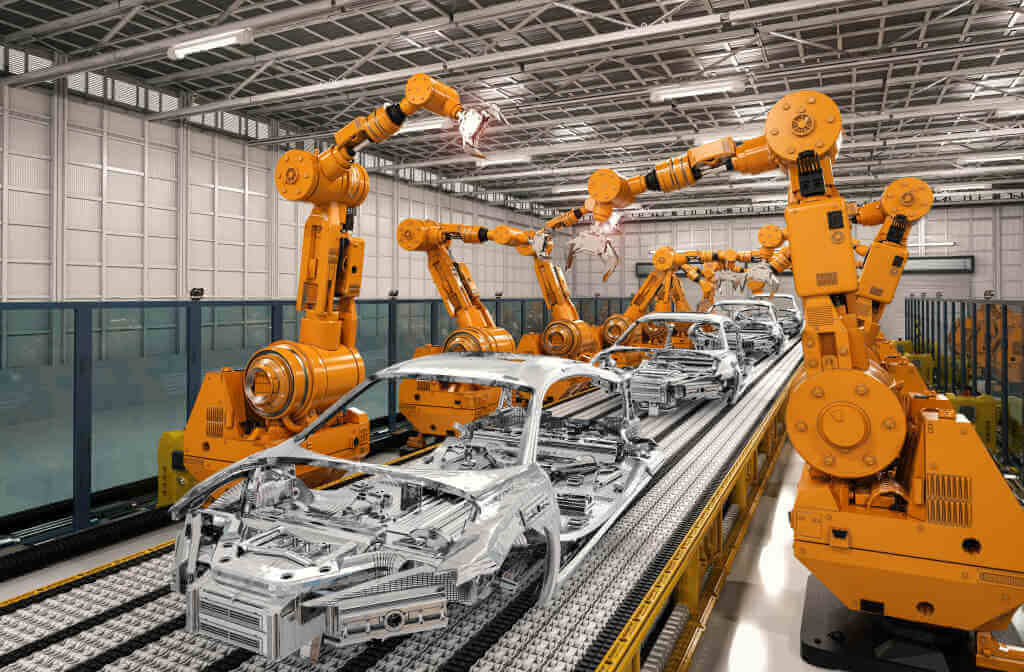
\includegraphics[width=10cm]{figures/IndustrialRobot.jpg}
  \caption{Robot công nghiệp [Nguồn: Internet]}
  \label{fig:RBCongNghiep}
\end{figure}

Bên cạnh đó, robot di động (mobile robot) truyền thống thực hiện các nhiệm vụ di chuyển trên quỹ đạo xác định trước. Robot di động cũng hoạt động dựa trên các khối chương trình được lập trình sẵn. Các phương pháp điều khiển như điều khiển bằng tay thông qua bảng điều khiển, qua sóng RF, wifi... hay di chuyển bám đường chỉ dẫn gắn ở dưới sàn, đọc mã QR, bar. Robot dạng này bị hạn chế về không gian hoạt động. Việc thiết lập, cấu hình nhà máy, không gian làm việc cho robot hoạt động hết sức tốn kém về chi phí và thời gian mà lại kém linh hoạt.

Ngày nay, robot có xu hướng đi ra khỏi không gian nhà máy, xuất hiện nhiều loại robot như: robot giải trí (\figurename{\ref{fig:rbMoi-a}}), robot dịch vụ cá nhân (\figurename{\ref{fig:rbMoi-b}}) (như máy tính cá nhân), robot trong y tế (\figurename{\ref{fig:rbMoi-c}}); các loại robot tự động trong công nghiệp như robot hái quả (\figurename{\ref{fig:rbMoi-d}}), phun thuốc trong nông nghiệp, robot thông minh tác hợp trong công nghiệp; robot đi tới các môi trường mà con người không tới được như trong lòng đất dưới nước, trên không, trong vũ trụ...
\begin{figure}
	\centering
	\subfloat[][]{
          \label{fig:rbMoi-a}
          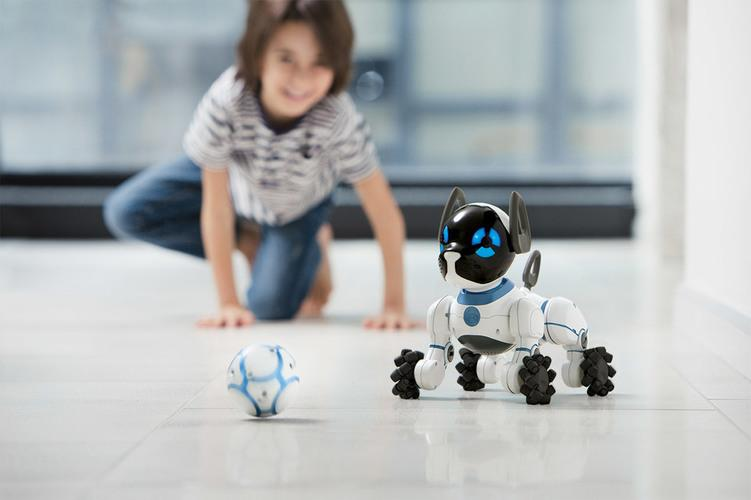
\includegraphics[height=5cm]{figures/c1_entertainmentRobot.jpg}}
        \subfloat[][]{
          \label{fig:rbMoi-b}
          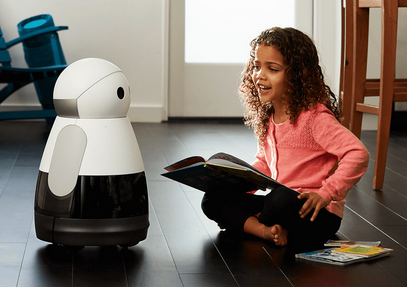
\includegraphics[height=5cm]{figures/c1_personalServiceRobot.png}}
        \hspace{8pt}
        \subfloat[][]{
          \label{fig:rbMoi-c}
          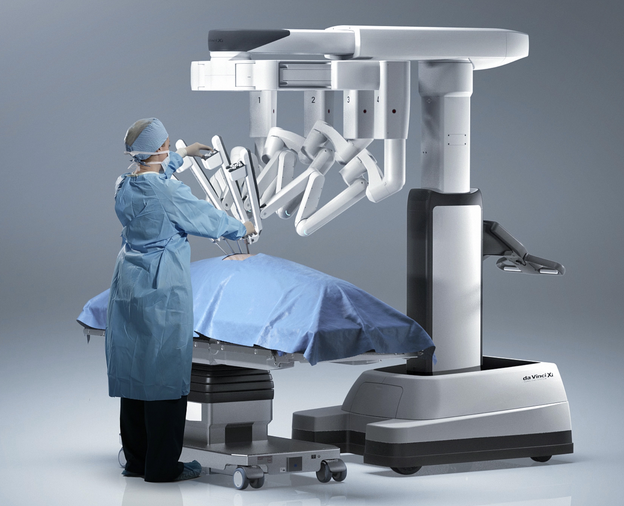
\includegraphics[height=4.6cm]{figures/c1_medicalRobot.png}}
        \subfloat[][]{
          \label{fig:rbMoi-d}
          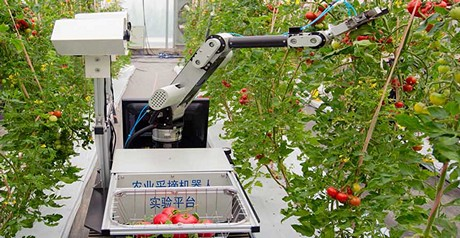
\includegraphics[height=4.6cm]{figures/c1_harvestingRobot.jpg}}
	\hspace{8pt}
	\caption[]{Một số loại robot mới}
	\label{fig:rbMoi}
\end{figure}

\begin{figure}[htp]
  \centering
  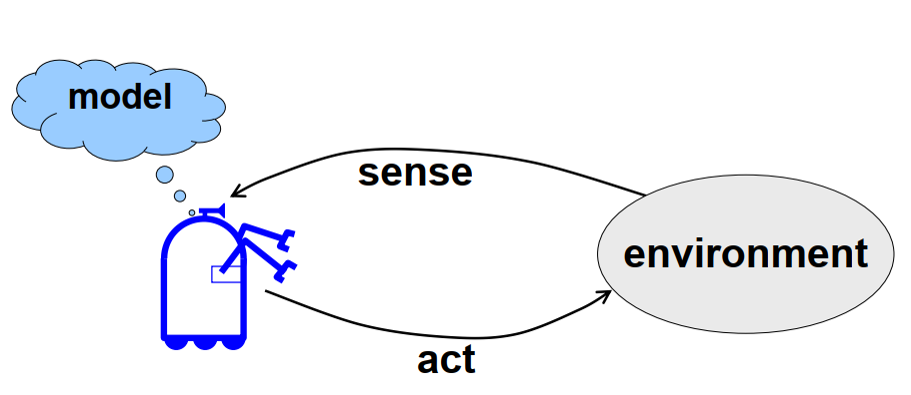
\includegraphics[width=12cm]{figures/c1_AutonomousRBModel.png}
  \caption{Mô hình hệ thống robot tự hành}
  \label{fig:MohinhRB}
\end{figure}

%Trong đó, hệ thống robot tự hành là một dạng robot điển hình cho thế hệ robot mới ngày nay và đang phát triển rất mạnh mẽ. Hệ thống robot tự hành là hệ thống hoạt động như mô hình \figurename{\ref{fig:MohinhRB}}: Robot cảm nhận môi trường thông qua hệ thống cảm biến. Mô hình hóa môi trường sau đó thực hiện các hành động phản ứng lại với môi trường. Các hoạt động cảm nhận môi trường như đo khoảng cách bằng cảm biến siêu âm, hồng ngoại, lidar hay ứng dụng deep learning để nhận dạng đồ vật, người... Các hành động phản ứng có thể là xây dựng bản đồ, thực hiện di chuyển, thực hiện tránh vật, gắp vật...

Robot tự hành thông minh là loại robot di động, có thể cảm nhận, mô hình hóa môi trường xung quanh nó. Thực hiện các hành động di chuyển mà không cần sự giám sát cũng như điều khiển trực tiếp từ con người (\figurename{\ref{fig:MohinhRB}}).

% Có nên thêm phần giới thiệu các robot dựa trên robot tự hành:

\section{Ứng dụng của robot tự hành thông minh}
\label{sec:ungdung}

Với sự thông minh và cực kì linh hoạt của nó, robot tự hành thông minh có rất nhiều ứng dụng. Về cơ bản, nó là nền tảng di chuyển cho tất cả các loại robot di động thông minh ngày nay. Một số sản phẩm ứng dụng trong nhà như:

\begin{itemize}
\item Các ứng dụng trong nhà như robot hút bụi thông minh, robot dịch vụ, robot vận chuyển trong các kho hàng\dots
\item Các ứng dụng ngoài trời như robot cắt cỏ, chăm sóc cây trồng...
\item Ở các không gian mà con người không tới được như robot thám hiểm dưới nước, trong lòng đất, trên không trung trên các hành tinh khác...
\item Tại các khu vực nguy hiểm như khu vực nhiễm chất phóng xạ, chữa cháy...
\item Và đặc biệt, robot giao hàng tự động, xe tự lái đang phát triển rất nhanh trong những năm gần đây 
\end{itemize}

\section{Các bài toán trên robot tự hành thông minh}

% - Nêu qua concept về điều khiển robot, tạo bản đồ, định vị, path planning, điều hướng, tránh vật cản
Một số bài toán chính trong robot tự hành như sau (\cite{Wise}):

\textbf{Cảm biến:} Robot tự hành thông minh cần một số loại cảm biến để có thể hiểu được môi trường, định vị và di chuyển tránh vật cản. 

Có rất nhiều loại cảm biến, để cảm nhận được đa dạng thông tin của môi trường. Có thể chia làm các nhóm như sau:
\begin{itemize}
\item Khoảng cách 1D: Cảm biến khoảng cách hồng ngoại, siêu âm
\item Khoảng cách 2D: Lidar
\item Cảm biến 3D: Có nhiều loại cảm biến 3D như Intel realsense, Microsoft Kinect, Asus Xction...
\item Ước tính trạng thái robot: GPS, IMU
\item Cảm biến lực, momen, cảm biến chạm...
\item Âm thanh, giọng nói như microphone, microphone array
\item Các loại camera 2D
\end{itemize}

\textbf{Odometry}: là bài toán sử dụng thông tin nhận được từ các cảm biến nhận biết sự di chuyển của robot để ước tính sự thay đổi vị trí của robot qua thời gian. Odometry được sử dụng trong hầu hết các robot tự hành.

\textbf{Định vị}: Bài toán định vị giúp trả lời câu hỏi robot đang ở đâu, từ đó có cơ sở để thực hiện các tác vụ khác như tạo bản đồ, xác định hướng di chuyển.

\textbf{Xây dựng bản đồ}: Dự trên dữ liệu từ các loại cảm biến, từ odometry và định vị robot, robot sử dụng các thuật toán để xây dựng bản đồ của môi trường.

\textbf{Điều hướng robot}: Từ bài toán định vị và khi có được bản đồ và nhiệm vụ di chuyển từ vị trí hiện tại tới một vị trí đích. Robot sẽ tính toán qũy đạo và điều khiển di chuyển tới đích.

\textbf{Tránh vật cản}: Trong quá trình di chuyển, robot phải phát hiện được các vật cản (bao gồm cả tĩnh và động) và tránh vật cản, sau đó thiết lập lại quỹ đạo di chuyển tới đích.

Vấn đề xuyên suốt trong các bài toán của robot tự hành thông minh đó là các dữ liệu đều không chắc chắn, các bài toán trên đều dựa vào các mô hình xác suất để mô hình hóa được trình bày trong tài liệu \cite{Sebastian2005}.

% Thêm một đoạn dẫn liên kết vào đây

\section{Các nghiên cứu tránh vật cản trong robot tự hành thông minh}
\label{sec:tranhVatCan_ref}

% Review các bài báo về tránh vật cản trong robot tự hành
% Chỉ ra các ưu, nhược điểm của các phương pháp như được nêu trong các bài báo trên
Khả năng phát hiện và tránh vật cản theo thời gian thực là rất quan trọng trong robot tự hành. Do đó có rất nhiều nghiên cứu về giải pháp cho vấn đề này. Có nhiều loại cảm biến được sử dụng, nhiều giải thuật được sử dụng. Các loại cảm biến sử dụng như cảm biến khoảng cách hồng ngoại, siêu âm với ứng dụng trên các thiết bị nhúng cấu hình thấp \cite{dongyue2013, Susnea2009}. Các phương pháp sử dụng cảm biến laser radar được trình bày trong \cite{Gao2019, Wu2015, Peng2015}. Các thuật toán phổ biến được dùng để phát hiện và tránh vật cản như Virtual Force Field (VFF) \cite{Borenstein1989}, Vector Field Histogram (VFH) \cite{Borenstein1991}, Dynamic Window Approach (DWA) \cite{Fox1997}\ldots

\subsection{Thuật toán Virtual Force Field (VFF)}

Được áp dụng cho điều khiển tránh vật cản trình bày trong \cite{Borenstein1988,Borenstein1989}. Ý tưởng của giải thuật này là tạo một ô lưới quanh robot. Khi có dữ liệu có vật cản từ cảm biến, ô tương ứng sẽ được đặt là bị chiếm dụng bởi vật cản với một tỉ số chiếm dụng (thể hiện cho sự không chắc chắn), nhiệm vụ của thuật toán là tính toán một lực để đưa robot xa khỏi ô bị chiếm dụng đó.


\begin{equation}
  F(i,j) = \frac{{F}_{cr}C(i,j)}{{d}^{2}(i,j)}\left [\frac{{x}_{t}-{x}_{0}}{d(i,j)}\dot{x} + \frac{{y}_{t}-{y}_{0}}{d(i,j)}\dot{y} 
  \right ]
\end{equation}
Trong đó: 

\begin{tabular}{ll}
  $F(i,j)$      & Lực ảo chống lại vật cản tại ô (i,j) \\
  ${F}_{cr}$    & Hằng số lực chống lại vật cản  \\
  $d(i,j)$      & Khoảng cách giữa ô (i,j) và robot \\
  ${C}_{i,j}$   & Độ chắc chắn tại ô (i,j)  \\
  ${x}_{0}, {y}_{0}$ & Tọa độ robot \\
  ${x}_{i}, {y}_{j}$ & Tọa độ của ô (i,j)
\end{tabular}

Lực ${F}_{r}$ đưa robot tránh khỏi các vật cản xuất hiện xung quanh robot là tổng của các lực tại mỗi ô lưới. 

\begin{equation}
  {F}_{r} = \sum\limits_{i,j}{F(i,j)}
\end{equation}

Trong khi đó, lực ${F}_{t}$ kéo robot đi từ điểm hiện tại tới điểm đích như sau: 

\begin{equation}
  {F}_{t} = {F}_{ct} \left [\frac{{x}_{t}-{x}_{0}}{d(t)}\dot{x} + \frac{{y}_{t}-{y}_{0}}{d(t)}\dot{y} 
  \right ]
\end{equation}

Trong đó: 

\begin{tabular} {ll}
  ${F}_{ct}$    & Hằng số lực kéo robot tới đích \\
  $d(t)$        & Khoảng cách giữa robot và điểm đích \\
  ${x}_{t}, {y}_{t}$ & Tọa độ của điểm đích
\end{tabular}

\begin{figure}[htp]
  \centering
  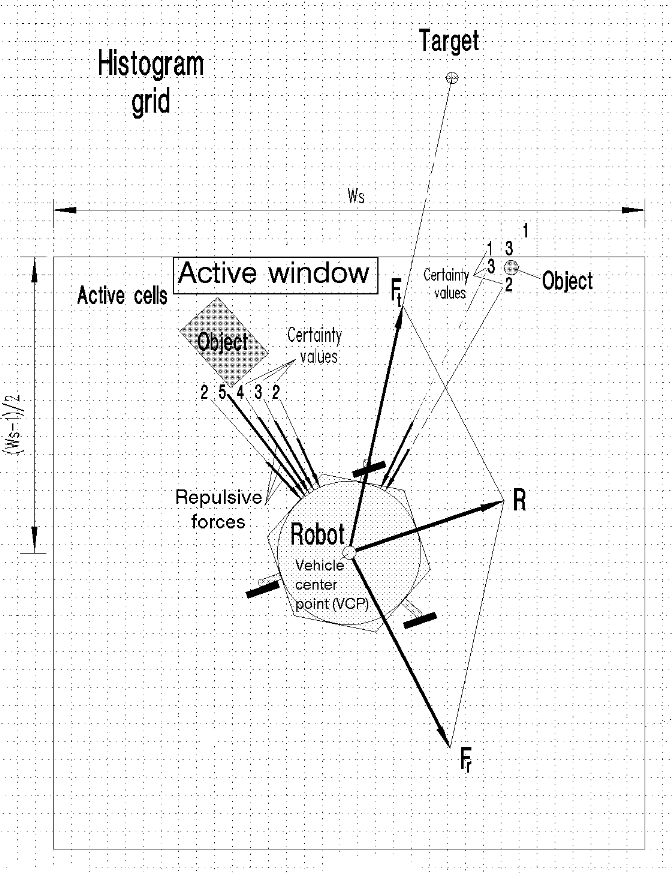
\includegraphics[width=0.5\linewidth]{figures/VFFconcept.png}
  \caption{Virtual Force Field \cite{Koren1991}}
  \label{fig:VFFconcept}
\end{figure}

Hợp lực của 2 loại lực này là lực chính kéo robot di chuyển.

\begin{equation}
  R = {F}_{t} + {F}_{r}
\end{equation}


Từ đó tính được hướng di chuyển của robot để điều khiển bánh xe di chuyển, đưa robot tới đích và tránh được vật cản. Theo \cite{Borenstein1988}, phương pháp này có một số ưu điểm như sau:
\begin{itemize}
  \item Phương pháp này không xác định được đường viền cạnh của vật cản, nhưng có thể xác định được cụm các vị trí có vật cản.
  \item Phương pháp này không yêu cầu robot phải dừng lại để thực hiện lấy dữ liệu và tính toán. Trong điều kiện lý tưởng, phương pháp này giúp robot có thể tránh được tất cả vật cản trong khi vẫn di chuyển với vận tốc tối đa.
  \item Việc cập nhật bản đồ lưới và điều hướng sử dụng bản đồ lưới là hai nhiệm vụ hoàn toàn không phụ thuộc vào nhau, nhưng có thể đồng bộ với nhau để tối ưu tính toán. 
  \item Phương pháp này có thể dễ dàng tích hợp nhiều loại cảm biến để bổ sung thông tin vào bản đồ ô lưới. 
\end{itemize}

Tuy nhiên, theo \cite{Koren1991}, phương pháp này có một số điểm hạn chế như: Các trường hợp mắc bẫy do cực tiểu địa phương, không thể di chuyển qua giữa các vật cản gần nhau, lưỡng lự khi có vật cản, lưỡng lự trong lối đi hẹp

Do đó, phương pháp Vector Field Histogram cải thiện các hạn chế của phương pháp Vector Force Field

\subsection{The Vector Field Histogram}
\label{sub:VFH}
Phương pháp VFH \cite{Borenstein1991} sử dụng kĩ thuật hai giai đoạn giảm dữ liệu và ba mức thể hiện dữ liệu:

\begin{itemize}
  \item Mức biểu diễn dữ liệu cao nhất giữ mô tả chi tiết của môi trường robot, bản đồ lưới 2 chiều được cập nhật liên tục theo thời gian thực như trong phương pháp VFF. 
  \item Mức ở giữa, một biểu đồ H một chiều được dựng quanh vị trí tức thời của robot. H bao gồm $n$ góc với độ rộng $\alpha$, phép chuyển đổi từ C sang H. 
  \item Mức biểu diễn dữ liệu thấp nhất là đầu ra của thuật toán VFH: các giá trị tham chiếu cho động cơ và bánh xe điều khiển robot. 
\end{itemize}

% \begin{figure}[htp]
%   \centering
%   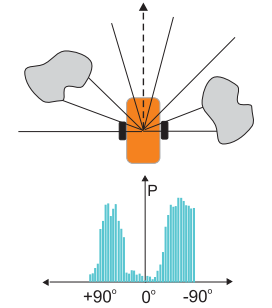
\includegraphics[]{figures/VFH.png}
%   \caption{Virtual Force Field \cite{Susnea2009}}
%   \label{}
% \end{figure}

\begin{wrapfigure}{r}{0.4\textwidth}
  \centering
  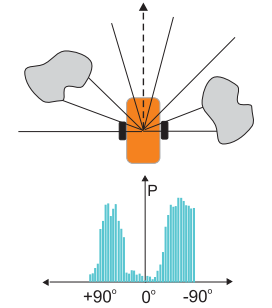
\includegraphics[width=0.4\textwidth]{figures/VFH.png}
  \caption{Vector Field Histogram \cite{Susnea2009}}
  \label{fig:VFH}
\end{wrapfigure}

Phương pháp này có thể phát hiện được lối đi đủ cho robot đi qua giữa các vật cản.  Phương pháp VFF dễ bị ảnh hưởng bởi sai số của cảm biến, với phương pháp này, sử dụng làm mịn biểu đồ H đã giảm trọng số của các giá trị sai ngẫu nhiên của cảm biến, do đó phương pháp này mạnh hơn phương pháp VFF. Vẫn bị hiện tượng mắc bẫy khi vào các trường hợp "dead-end" (đường cụt) do sử dụng phương pháp cục bộ. Tốc độ di chuyển tối đa khi điều khiển robot bằng VFH bị giới hạn bởi tốc độ lấy mẫu của cảm biến. 

Dựa trên phương pháp này, \cite{Ulrich1998} đã đề xuất phương pháp được gọi là VFH+ thực hiện 4 giai đoạn giảm dữ liệu từ bản đồ lưới chiếm dụng hai chiều xuống thành dữ liệu điều khiển hướng di chuyển của robot. Sử dụng một số cải tiến để giúp robot có thể di chuyển tốt hơn.
  
\subsection{Phương pháp "Bong bóng phản ứng" tránh vật cản}

\begin{wrapfigure}{r}{0.5\textwidth}
  \centering
  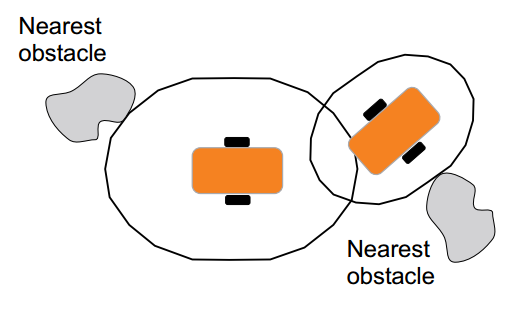
\includegraphics[width=0.5\textwidth]{figures/bubble-band.png}
  \caption{Bong bóng phản ứng \cite{Susnea2009}}
  \label{fig:bubble-band}
\end{wrapfigure}

Phương pháp này được đề xuất trong \cite{Quinlan1993}, phương pháp này định nghĩa một "bong bóng" bao quanh robot thể hiện không gian lớn nhất có thể di chuyển mà không gặp vật cản. Hình dạng và kích thước của bong bóng được xác định đơn giản dựa trên hình dạng vật lý của đế robot và từ thông tin của cảm biến (như \figurename{\ref{fig:bubble-band}}).

\begin{figure}
	\centering
	\subfloat[][]{
          \label{fig:bb-computeAngle}
          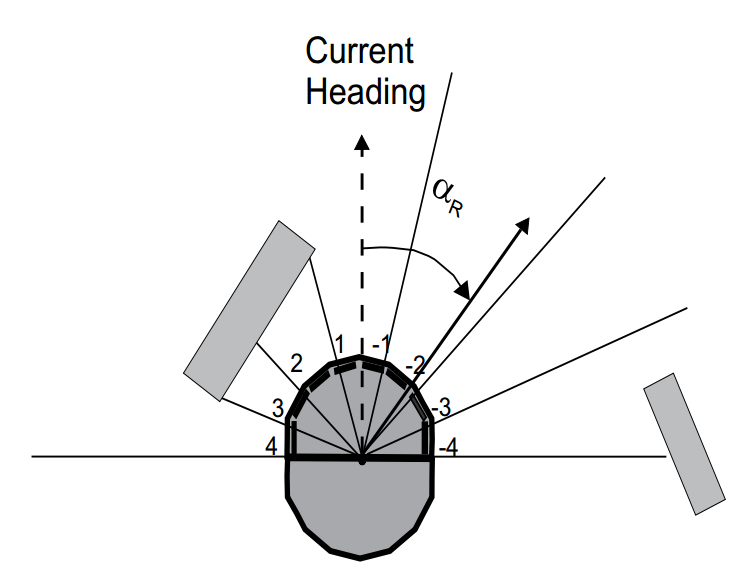
\includegraphics[width=0.45\textwidth]{figures/computeReboundAngle.png}}
        \subfloat[][]{
          \label{fig:bb-reboudProcess}
          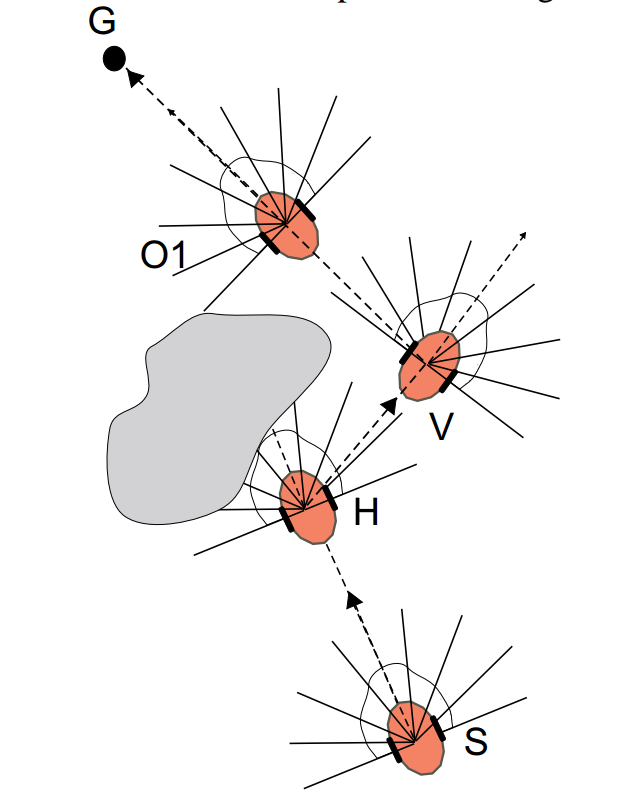
\includegraphics[width=0.45\textwidth]{figures/rebound.png}}
	\hspace{8pt}
	\caption{Phương pháp bong bóng phản ứng động}
	\label{fig:bubbleRebound}
\end{figure}

Một phương pháp cải tiến được đề xuất trong \cite{Susnea2010}. Tác giả đã cải tiến hình dạng của bong bóng, không phải là hình dạng cố định như trong \cite{Quinlan1993} mà hình dạng và kích thước được điều chỉnh liên tục dựa vào tốc độ di chuyển của robot. Khi các cảm biến phát hiện vật cản nằm trong giới hạn của bong bóng phản ứng, một thuật toán được dùng để xác định hướng của vật cản so với hướng di chuyển của robot \figurename{\ref{fig:bb-computeAngle}}. Một quá trình di chuyển của robot sử dụng phương pháp này được minh họa tại \figurename{\ref{fig:bb-reboudProcess}}.

Cũng theo tác giả \cite{Susnea2010}, phương pháp này có ưu điểm là có thể triển khai trên các thiết bị giá thành thấp, chi phí tính toán thấp nhưng có thể hoạt động theo thời gian thực. Tuy nhiên, nó cũng có một số điểm hạn chế như quá trình di chuyển chưa mượt, robot khó xử lý khi gặp nhiều vật cản đồng thời \dots

\section{Nội dung nghiên cứu}

% Chốt lại nội dung nghiên cứu gồm 2 nội dung:
% - Điều khiển robot ứng dụng SLAM trên nền tảng hệ điều hành ROS
% - Sử dụng Multi-sensor để tăng cường phát hiện và tránh vật cản cho robot
% - Trình bày vắn tắt nội dung của các chương.

Với mong muốn tiếp cận với công nghệ thế giới trong lĩnh vực robot tự hành, xe tự lái, luận văn này thực hiện 2 nhiệm vụ chính:
\begin{itemize}
  \item Cấu hình robot ứng dụng SLAM trên nền tảng hệ điều hành ROS
  \item Tăng cường phát hiện và tránh vật cản cho robot bằng đa cảm biến.
\end{itemize}

%%===========================
\chapter{Cơ sở lý thuyết}
\label{chap:1cslt}
\section{Bài toán về nhiễu trong robot tự hành}


\section{Bài toán SLAM 2D}

\section{Bài toán tạo định vị, tạo bản đồ, điều hướng và tránh vật cản}

\section{Hệ điều hành robot ROS và các ứng dụng}

% Tóm gọn nội dung giới thiệu về ROS và các ứng dụng trong khuôn khổ của luận văn này.

%% ===================
%%% Local Variables:
%%% mode: latex
%%% TeX-master: "../LuanVanThS_v1.0_main"
%%% End:

\chapter{Điều khiển và cải tiến tránh vật cản cho robot}}
%===================

\section{Đặt vấn đề}
%------------------

% Nhắc lại vấn đề ở phần cuối chương 1
Công nghệ SLAM là công nghệ cốt lõi trong robot tự hành thông minh, hiện nay công nghệ SLAM 2D chiếm phần lớn trong các ứng dụng do tính đơn giản, giá thành hợp lý. Tuy nhiên, với SLAM 2D, robot chỉ có thể tạo được bản đồ và di chuyển, tránh vật cản khi có thông tin về vật cản đó trên một mặt phẳng mà LIDAR quét được. Trong thực tế, môi trường hoạt động của chúng có nhiều loại vật thể có hình dạng, kích thước và chiều cao khác nhau.

Để giải quyết vấn đề này, có một số phương pháp như:
\begin{itemize}
    \item Thêm một số tầng cảm biến khác theo chiều cao thân robot như robot RHINO (\cite{Buhmann1995})
    \item Sử dụng cảm biến LIDAR 3D (\cite{Pierzchala2018})
    \item Ứng dụng visual-based SLAM (\cite{Chen2000, Mittal2019})
\end{itemize}

Các phương pháp trên có nhược điểm là chi phí thiết bị cao, chi phí tính toán lớn do robot phải xử lý lượng lớn dữ liệu đầu vào. Trong luận văn này , để đảm bảo robot có thể hoạt động được theo thời gian thực và tích hợp trên hệ thống sẵn có, tác giả sử dụng phương pháp tích hợp thêm một tầng cảm biến khoảng cách hồng ngoại để phối hợp với Lidar và cảm biến siêu âm có sẵn trên robot để hỗ trợ và tăng cường tránh vật cản cho robot. Tác giả thực hiện một số nhiệm vụ như sau:

\begin{itemize}
    \item Thiết kế mạch lấy dữ liệu cảm biến
    \item Lập trình lấy dữ liệu và xử lý dữ liệu từ các cảm biến khoảng cách hồng ngoại
    \item Đề xuất giải thuật điều khiển tránh vật cản bằng hệ thống cảm biến khoảng cách hồng ngoại.
    \item Phối hợp để phân quyền điều khiển robot
    \item Tích hợp tín hiệu từ cảm biến để cập  nhật dữ liệu vật cản vào bản đồ di chuyển của robot
    \item Đánh giá kết quả và hiệu quả của hệ thống
\end{itemize}

\section{Giới thiệu nền tảng robot}
\label{sec:RobotIntro}
% - Kiến trúc phần cứng của robot
% - Ứng dụng hệ điều hành ROS
% - Các bài toán điều khiển trên rb

Luận văn này được thực hiện trên nền tảng robot di động EAI Dashgo D1 \figurename{ \ref{fig:dashgoD1}} là một nền tảng robot di động thông minh được sản xuất phục vụ nghiên cứu về robot tự hành và Hình \ref{fig:airhustbot} là robot đang trong quá trình phát triển thành robot dịch vụ thông minh.

% \subsection{Phần cứng}

% \begin{figure}[htp]
% 	\centering
% 	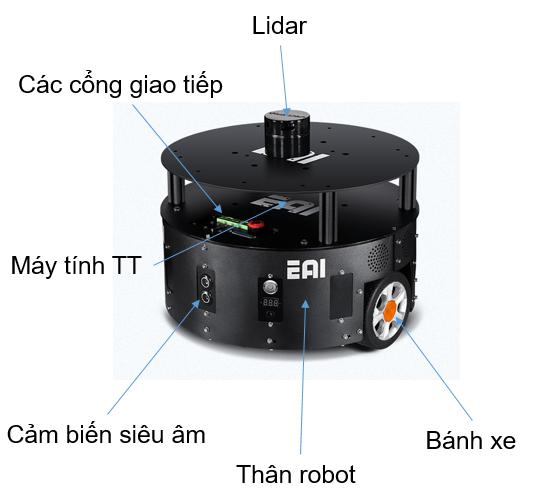
\includegraphics[width=0.7\linewidth]{figures/dashgoD1.JPG}
% 	\caption{Nền tảng robot di động Dashgo D1}
% 	\label{fig:dashgoD1}
% \end{figure}

\begin{figure}[htbp]
    \centering
    \subfloat[][]{
        \label{fig:dashgoD1}
        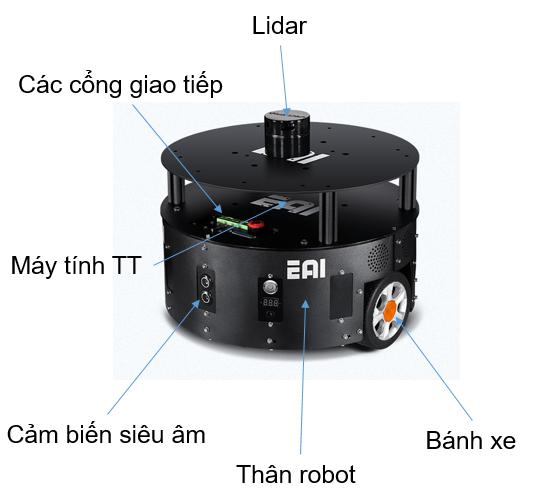
\includegraphics[width=0.5\linewidth]{figures/dashgoD1.JPG}}
    \subfloat[][]{
        \label{fig:airhustbot}
        \includegraphics[width=0.4\linewidth]{figures/airhustbot.png}}
    \caption{Nền tảng robot di động}
    \label{fig:platformRobto}
\end{figure}

Robot có cấu tạo gồm 3 phần chính: Phần chân đế thực hiện chức năng di chuyển, phần cảm biến và phần điều khiển trung tâm.

\begin{figure}[htbp]
	\centering
	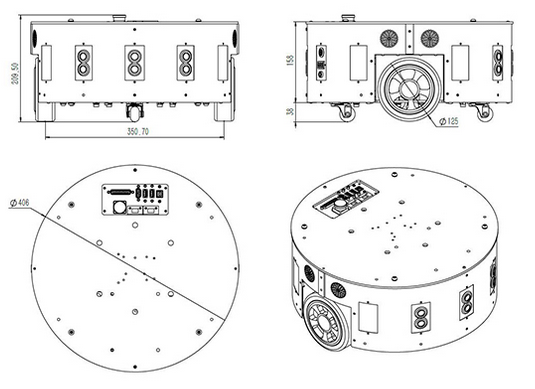
\includegraphics[width=0.7\linewidth]{figures/dashgo_base.png}
	\caption{Cấu tạo phần chân đế}
	\label{fig:dashgoBase}
\end{figure}

\subsection{Phần chân đế}
Phần chân đế có cấu tạo gồm hai bánh chủ động và 2 bánh xe bị động (\figurename{ \ref{fig:dashgoBase}}). Động cơ có gắn encoder độ chính xác cao để phản hồi vị trí. Phần chân đế được điều khiển bởi mạch điều khiển được mở rộng từ mạch arduino kết hợp với các module điều khiển bánh xe. Hoạt động của robot nhờ nguồn điện 12V từ acquy với thời gian sạc đầy khoảng 4 tiếng.

\subsection{Phần cảm biến}
Robot được trang bị bốn cảm biến siêu âm và một cảm biến LIDAR. Bốn cảm biến siêu âm sử dụng cho mục đích tránh vật cản. Nguyên lý hoạt động của cảm biến siêu âm như sau:
\begin{itemize}
    \item Đầu phát của cảm biến phát ra sóng siêu âm
    \item Sóng siêu âm bị dội lại khi có vật cản
    \item Thực hiện đo khoảng cách từ lúc phát tới lúc nhận được sóng dội lại, tính toán dựa trên tốc độ di chuyển sóng âm trong không khí ta tính được khoảng cách từ cảm biến tới vật.
\end{itemize}
Cảm biến siêu âm có các ưu điểm như không bị ảnh hưởng bởi màu sắc của vật, hoạt động tốt trong môi trường tối, tiêu tốn ít năng lượng và dễ dàng kết nối với các vi điều khiển. Tuy nhiên nó cũng có các điểm hạn chế như giới hạn khoảng cách đo được, độ phân giải và tần số đo thấp do đó nó không phù hợp với các ứng dụng có vật đích di chuyển nhanh. Cảm biến siêu âm không hoạt động được với các bề mặt không bằng phẳng, các bề mặt hấp thụ âm thanh.

Cảm biến YDLIDAR G4 sử dụng tia laser sử dụng đạt tiêu chuẩn an toàn FDA Class 1 \footnote{Tiêu chuẩn Laser FDA Class 1: Được xem là không gây nguy hiểm. Mức độ nguy hiểm tăng khi nhìn qua kính hội tụ quang học như kính lúp, kính hiển vi. Theo \url{www.fda.gov}}.
Cảm biến tích hợp một động cơ để quay quét mắt laser ${360}^{o}$ với tần số quét từ 5-12Hz. Đo khoảng cách bằng laser với giải đo từ 0.10 - 16m với tần số lấy mẫu có thể đạt 9000Hz.
Cảm biến này được sử dụng cho việc tạo bản đồ, điều hướng và tránh vật cản.


\subsection{Hệ thống phần mềm} \label{sub:software-architecture}
%       - Cấu trúc phần mềm: Linux-> ROS-> Package -> Subpackage
%       - Quy trình thực hiện một ứng dụng di chuyển tới các vị trí xác định trong văn phòng: Tạo bản đồ: gmapping -> Di chuyển trong bản đồ, dùng rviz (giống Hand-on)

\begin{figure}[htbp]
    \centering
    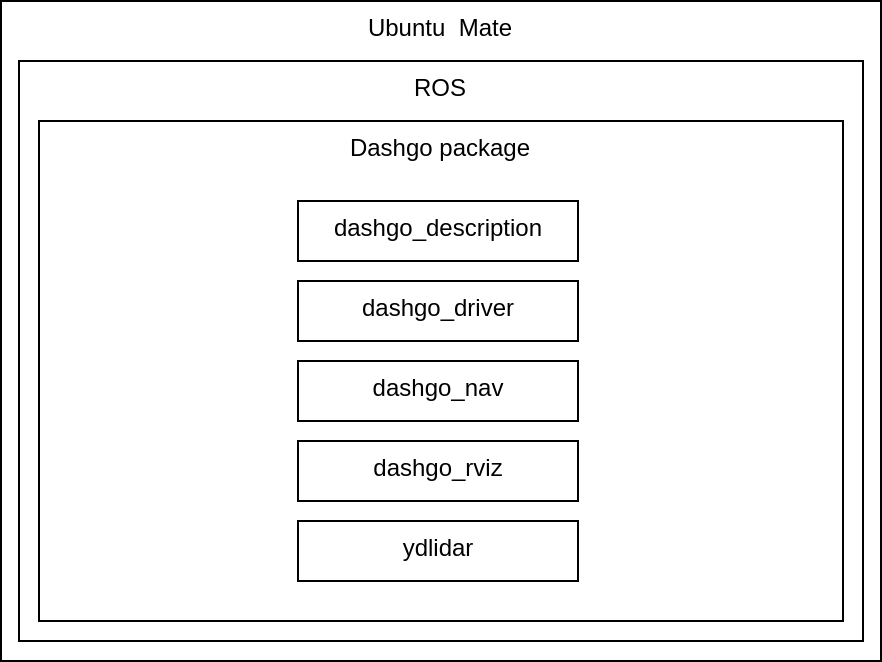
\includegraphics[width=0.7\linewidth]{figures/dashgo-architecture.png}
    \caption{Kiến trúc phần mềm điều khiển robot trên Dashgo D1}
    \label{fig:dashgo-architecture}
\end{figure}

Robot sử dụng mạch Raspberry Pi 3 làm bộ điều khiển trung tâm. Chạy hệ điều hành robot ROS Kinetic trên nền tảng Ubuntu MATE 16.04. Để thực hiện các chức năng cơ bản như định vị, tạo bản đồ, di chuyển tới vị trí xác định trong bản đồ, tránh vật cản trong quá trình di chuyển, robot cần phải được cài đặt gói chương trình dashgo được cung cấp bởi nhà sản xuất.
\figurename{ \ref{fig:dashgo-architecture}} mô tả kiến trúc phần mềm trên Dashgo D1. Trong đó:
\begin{itemize}
    \item \codeword{dashgo_description} là gói chứa các mô tả của robot, được dùng trong hiển thị Rviz và mô phỏng robot trong Gazebo.
    \item \codeword{dashgo_driver} chứa các thông số cấu hình và chương trình driver để điều khiển robot.
    \item \codeword{dashgo_nav} chứa các chương trình điều khiển robot, bao gồm \codeword{gmapping} để tạo bản đồ môi trường và \codeword{navigation} để thực hiện di chuyển tự động trong bản đồ.
    \item \codeword{dashgo_rviz} chứa các file mẫu rviz của một số tác vụ cơ bản.
    \item \codeword{dashgo_tools} chứa các công cụ để làm việc với robot.
    \item \codeword{ydlidar} là gói quản lý, driver của YDLIDAR.
\end{itemize}

\section{Điều khiển Dashgo robot}
%TODO:
% <<\textit{1. Các bước thực hiện tạo bản đồ, lưu bản đồ bằng gmapping -> Navigation: ước tính vị trí, di chuyển tới các điểm xác định trong bản đồ\\}
% \textit{2.Đánh giá hoạt động của robot}>>

Dashgo D1 ứng dụng giải thuật SLAM và hoạt động trên nền tảng hệ điều hành ROS.
Hai chức năng chính là tạo bản đồ môi trường mới và điều hướng trong môi trường đã biết.

\subsection{Quy trình thực hiện}

\textbf{Tạo bản đồ:} Với một môi trường chưa biết trước, việc đầu tiên là phải tạo bản đồ.
Chương trình tạo bản đồ được tạo sẵn trong file \codeword{gmapping.launch}

\begin{lstlisting}
$ roslaunch dashgo_nav gmapping.launch
\end{lstlisting}

Chương chương trình này sẽ gọi tới một số chức năng khác như driver điều khiển chân đế \codeword{driver.launch}, driver lidar \codeword{lidar.launch}, chạy thuật toán và khai báo các thông số tại \codeword{gmapping_base.launch}

Sau khi chạy file \codeword{gmapping.launch}, bật Rviz lên để xem vị trí của robot và bản đồ.
\begin{lstlisting}
$ roslaunch dashgo_rviz view_navigation.launch
\end{lstlisting}
%TODO: đặt hình ảnh rviz vào đây.


Sử dụng công cụ di chuyển robot bằng tay để thu thập thông tin tạo bản đồ của môi trường. Chúng ta có thể sử dụng bàn phím hoặc app để di chuyển robot. Cho robot di chuyển trong toàn bộ môi trường để thực hiện thu thập thông tin cho bản đồ. Theo dõi trực quan trên Rviz để quan sát bản đồ tạo được.
\begin{lstlisting}
$ rosrun dashgo_tools teleop_keyboard.py
\end{lstlisting}

Sau đó lưu bản đồ lại bằng lệnh:
\begin{lstlisting}
$ cd dashgo_nav/maps
$ rosrun map_server map_saver -f <Ten ban do>
\end{lstlisting}

\begin{figure}[htbp]
    \centering
    \subfloat[]{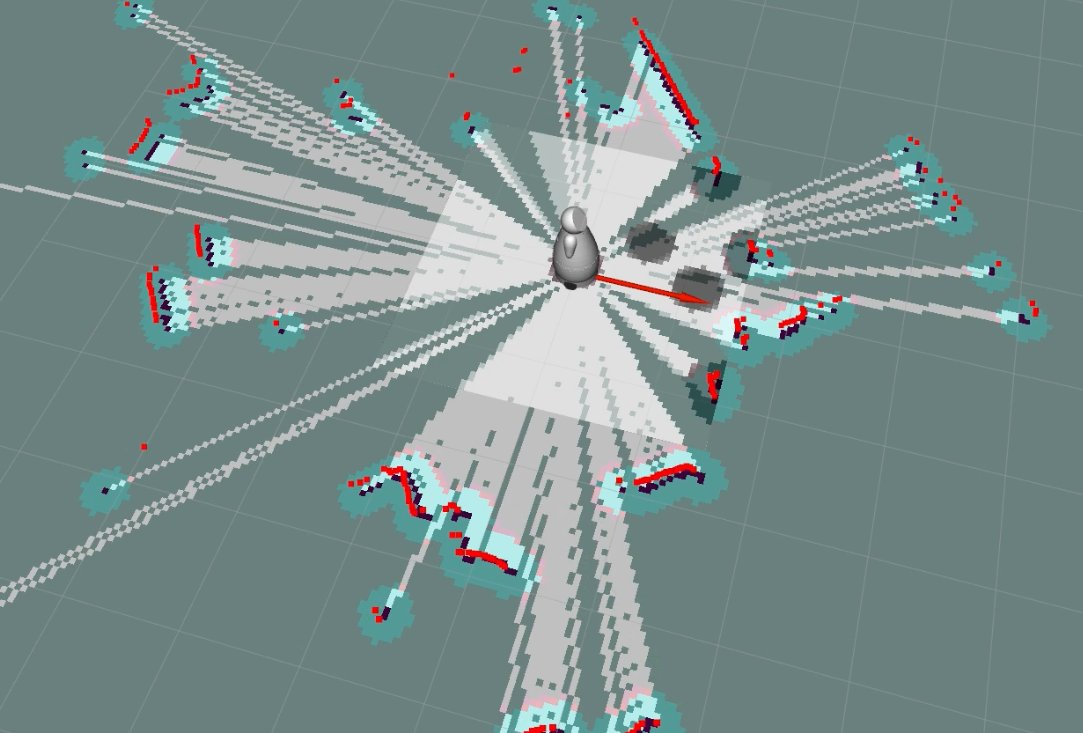
\includegraphics[width=0.75\linewidth]{figures/RB_mapping_start.jpg}}
    \hspace{8pt}
    \subfloat[]{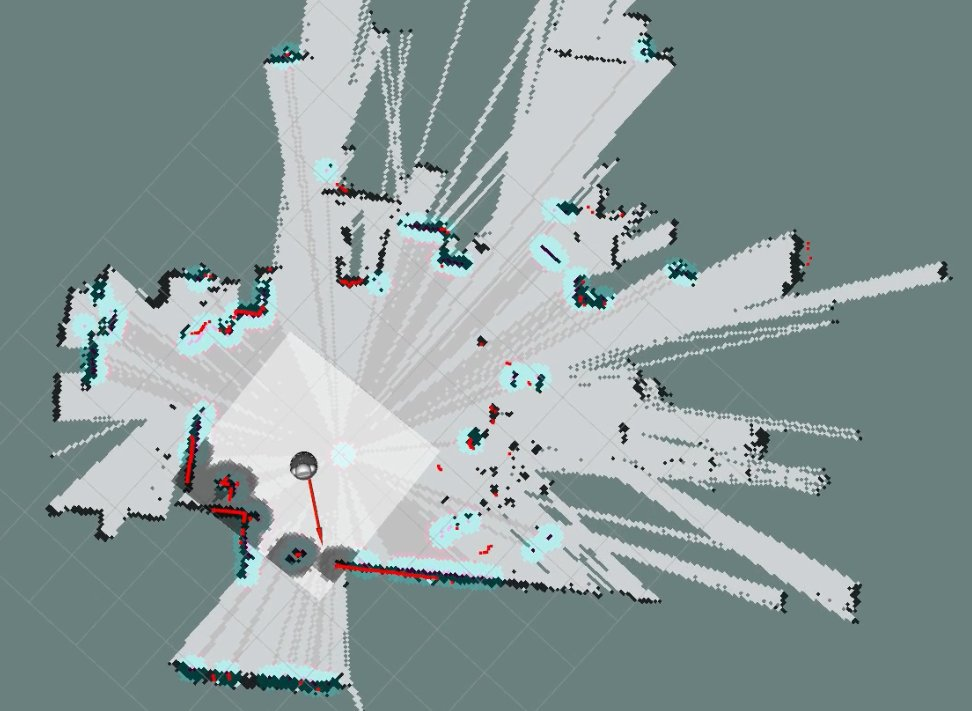
\includegraphics[width=0.75\linewidth]{figures/RB_mapping_end.jpg}}
    \caption[Robot đang tạo bảo đồ thể hiện trên Rviz]{Robot đang tạo bảo đồ thể hiện trên Rviz. Hình a thể hiện lúc bắt đầu tạo bản đồ, hình b là sau khi quét bản đồ xong.}
    \label{fig:mapping}
\end{figure}

\textbf{Điều hướng:} Chương trình này sử dụng bản đồ đã được lưu, sử dụng thuật toán amcl để định vị và điều hướng trong bản đồ đã biết.
\begin{lstlisting}
$ roslaunch dashgo_nav navigation.launch
\end{lstlisting}

Bật Rviz để xem trên bản đồ và thực hiện một số thao tác điều khiển cũng như theo dõi robot:
\begin{lstlisting}
$ roslaunch dashgo_rviz view_navigation.launch
\end{lstlisting}
%TODO: Thêm hình ảnh rviz lúc di chuyển
Trên giao diện Rviz, chúng ta sử dụng công cụ \codeword{2D Pose Estimate} để định vị lại vị trí của robot trong bản đồ bằng tay.
Bởi vì khi mới khởi tạo, robot chưa có đủ thông tin để tự định vị nó đang ở đâu trong bản đồ. Bước định vị bằng tay này không cần quá chính xác bởi vì sau khi robot di chuyển nó sẽ tự mình định vị và điều chỉnh vị trí của robot trong bản đồ. Sau đó, để điều hướng robot đến một điểm bất kì, chúng ta sử dụng công cụ \codeword{2D Nav Goal}. Ngoài ra, trên giao diện Rviz chúng ta còn có thể thấy các thông tin về: vị trí của robot, bản đồ, costmap\dots

\begin{figure}[htbp]
    \centering
    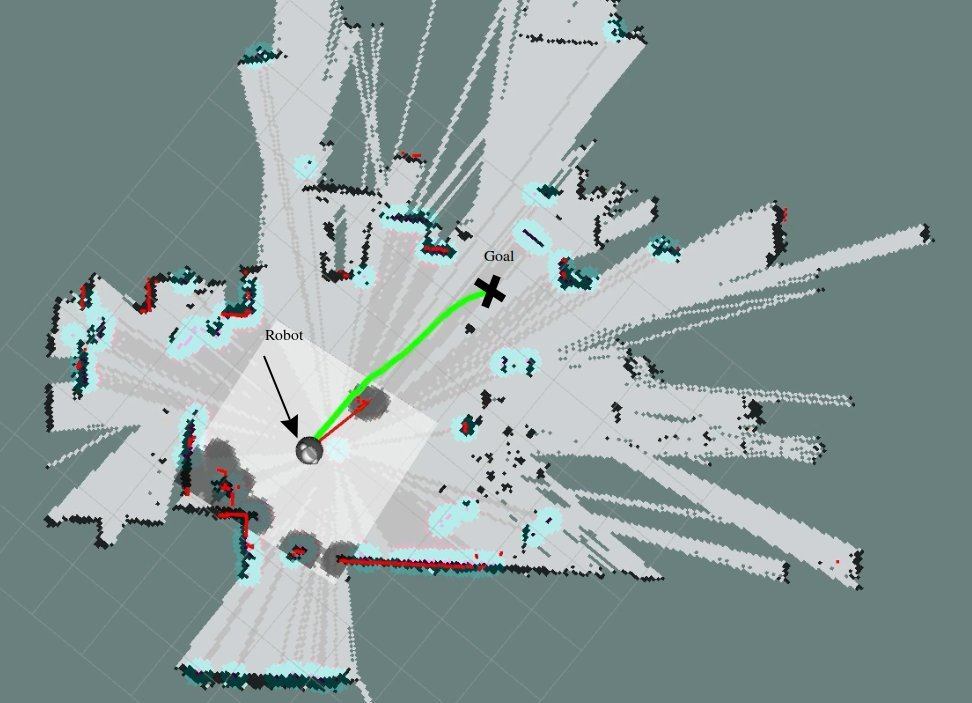
\includegraphics[width=0.75\linewidth]{figures/RB_navi_in_map.jpg}
    \caption{Robot di chuyển tới đích trong bản đồ}
    \label{fig:navigation}
\end{figure}

Hình \ref{fig:mapping} thể hiện quá trình tạo bản đồ của robot.
Hình \ref{fig:navigation} thể hiện robot đang di chuyển tới vị trí đích xác định trong bản đồ. Đường màu xanh lá là đường đi dự kiến được tính toán dựa trên bản đồ giá trị (costmap).
Để di chuyển tới vị trí đích xác định trong bản đồ. Robot sẽ dựa vào bản đồ toàn cục để tính được một quỹ đạo di chuyển với chi phí di chuyển thấp nhất từ vị trí đang đứng tới vị trí đích.
Đồng thời, một bản đồ địa phương là một ô lưới quanh robot. Trong bản đồ địa phương này, robot sẽ sử dụng tín hiệu từ các cảm biến để đánh dấu vật cản vào bản đồ để tránh vật cản đó.

\subsection{Đánh giá hoạt động của robot}
%FIXME: Đánh giá thêm
% Trong luận văn này, tác giả thực hiện 2 nhiệm vụ chính: Làm chủ điều khiển robot di động và cải tiến tránh vật cản bằng cảm biến khoảng cách hồng ngoại.

Với nền tảng robot hiện tại, hệ thống robot thực hiện được một số chức năng như sau:

\begin{itemize}
    \item Tạo bản đồ môi trường mới
    \item Di chuyển trong môi trường đã biết, điều hướng tới đích được cho.
    \item Tránh vật cản trong quá trình di chuyển.
\end{itemize}

Tuy nhiên bên cạnh đó cũng có một số hạn chế như sau:

\begin{itemize}
    \item Robot chỉ phát hiện và tránh vật cản được ở hai tầng cảm biến hiện tại (tương ứng với mặt phẳng đi qua cảm biến siêu âm và mặt phẳng quét của cảm biến LIDAR). Khi đó robot sẽ có một số hạn chế khi di chuyển trong môi trường có các vật có hình dạng khác nhau như bàn, ghế xoay\dots
    \item Cảm biến siêu âm tránh vật cản không phát hiện được vật cản có bề mặt hấp thụ sóng âm thanh
    \item Cảm biến laser sử dụng cho nhiệm vụ định vị, điều hướng và cả tránh vật cản, vì vậy chi phí tính toán cao và thường phản ứng chậm với vật cản động.
\end{itemize}


\section{Cải tiến hệ thống tránh vật cản cho robot}
\label{sec:caitienhethongtranhvatcan}
% - Lắp thêm cảm biến và xử lý dữ liệu cảm biến
% - Trình bày giải thuật đề xuất
% - Áp dụng giải thuật phát hiện và tránh vật cản
% - Phối hợp các tầng cảm biến và phân quyền điều khiển robot

% \subsection{Đặt vấn đề}

Từ các hạn chế của robot hiện tại và với mục tiêu robot hoạt động hiệu quả trong môi trường biến động, tác giả đề xuất phương án bổ sung thêm một tầng cảm biến để phát hiện và tránh vật cản. Hệ thống này sử dụng một số cảm biến khoảng cách hồng ngoại, chi phí thiết bị và chi tính toán thấp để dễ dàng tích hợp được vào robot, phối hợp cùng với hai tầng cảm biến có sẵn nhưng vẫn đảm bảo robot hoạt động ổn định theo thời gian thực. Robot có thể phát hiện và tránh được đa dạng vật cản hơn. Dựa trên các kết quả tham khảo ở \ref{sec:tranhVatCan_ref} tác giả đề xuất một mô hình giải thuật mới.

\subsection{Phần cứng}

% \begin{figure}[htbp]
    %     \centering
    %     \subfloat[][]{
        %         \label{fig:arduino}
        %         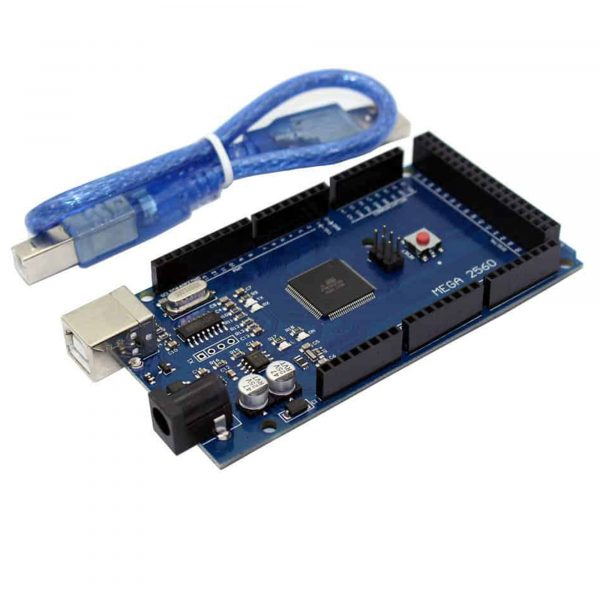
\includegraphics[width=0.5\linewidth]{figures/arduinoMega.jpg}}
        %     \subfloat[][]{
            %         \label{fig:irSharp}h
%         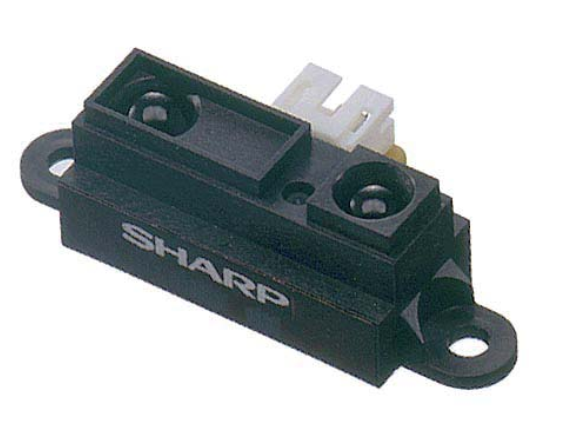
\includegraphics[width=0.4\linewidth]{figures/IRsharp.png}}
%     \caption{Phần cứng sử dụng}
%     \label{fig:components}
% \end{figure}

Hệ thống gồm một số cảm biến hồng ngoại IR Sharp GP2Y0A21YK0F và mạch Arduino Mega 2560. Vị trí các cảm biến được bố trí như \figurename{ \ref{fig:IR_layout}}.

\begin{figure}[htbp]
	\centering
	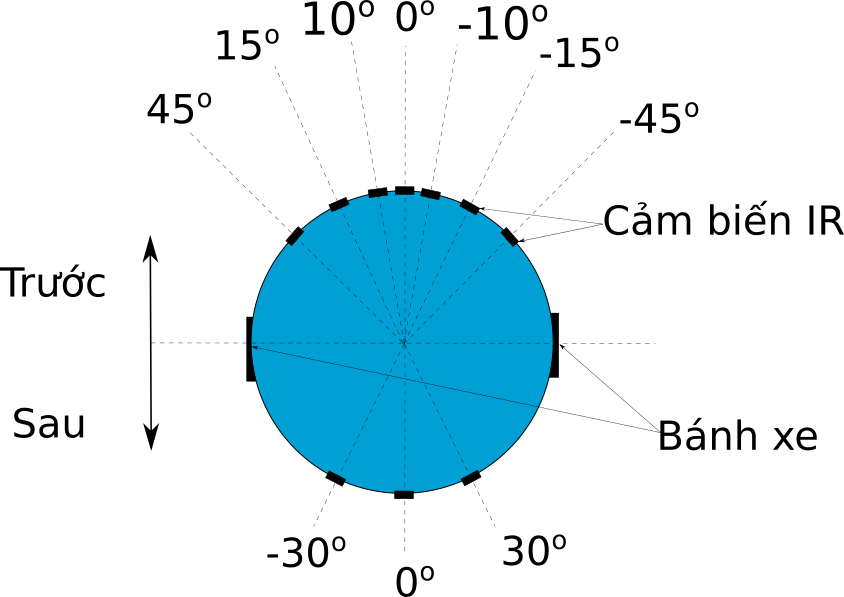
\includegraphics[width=0.7\linewidth]{figures/IR_layout.png}
	\caption{Sơ đồ bố trí cảm biến}
	\label{fig:IR_layout}
\end{figure}

\begin{figure}[htbp]
    \centering
    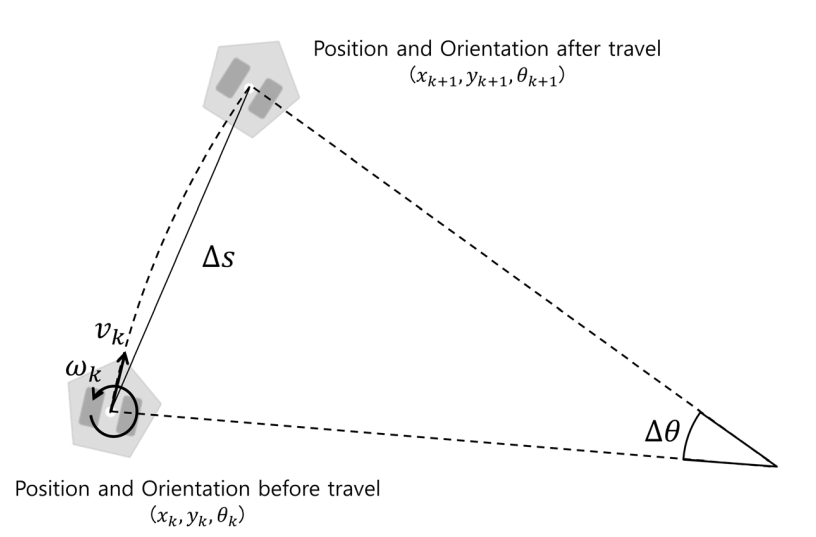
\includegraphics[width=0.7\linewidth]{figures/dead-reckoning.png}
    \caption{Dead reckoning \cite{pyo2017ros}}
    \label{fig:dead-reckoning}
\end{figure}

Trong quá trình di chuyển, robot có thể tiến và lùi vì vậy cần phải đặt cảm biến ở cả trước và phía sau robot.
Robot sử dụng hai bánh dẫn động chính và di chuyển trên mặt phẳng, do vậy chuyển động của robot được quy về hai thông số vận tốc dài $v$ và vận tốc góc $\omega$ theo phương pháp ước tính trạng thái robot dead-reckoning Hình \ref{fig:dead-reckoning} \cite{pyo2017ros}.
Do đó tác giả đề xuất phương án mới đặt cảm biến dày hơn ở khu vực chính giữa và thưa ra hai bên như \figurename{ \ref{fig:IR_layout}}.

\subsection{Xử lý dữ liệu cảm biến}

\begin{figure}[htbp]
    \centering
    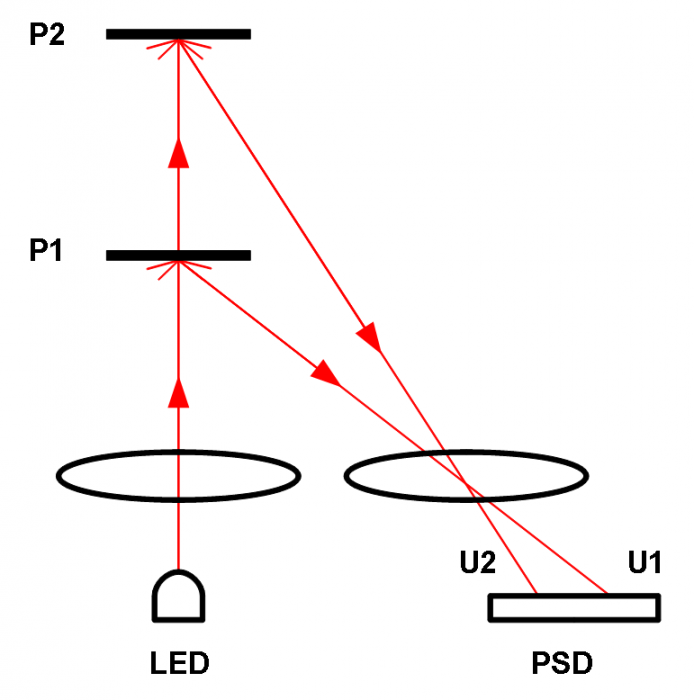
\includegraphics[width=0.5\linewidth]{figures/sensor_ir_distance_principle.png}
    \caption{Cơ chế hoạt động của cảm biến khoảng cách hồng ngoại}
    \label{fig:sensor_ir_distance_principle}
\end{figure}

\begin{figure}[htbp]
    \centering
    \subfloat[][]{
        \label{fig:irSharp-vol-distance}
        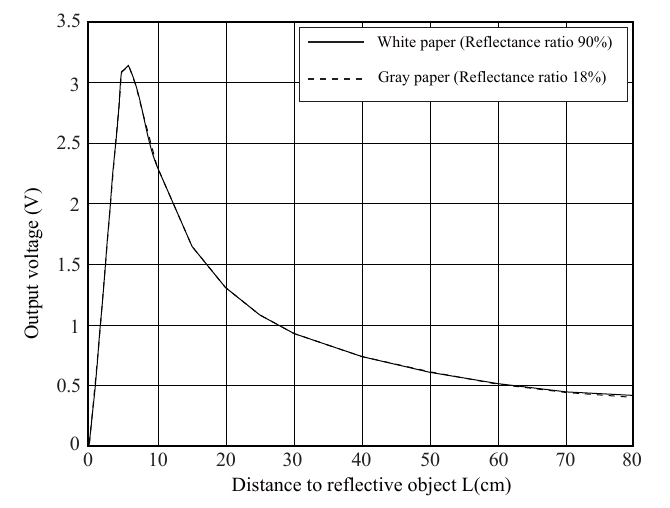
\includegraphics[width=0.5\linewidth]{figures/irSharp-vol-distance.png}
    }
    \subfloat[][]{
        \label{fig:irSharp-vol-distance_2}
        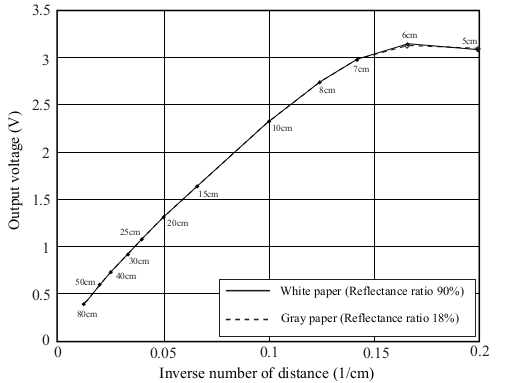
\includegraphics[width=0.5\linewidth]{figures/irSharp-vol-distance_2.png}
    }
    \caption{Mối liên hệ giữa khoảng cách và điện áp}
    \label{fig:irSharp-vol-distance}
\end{figure}

Cảm biến khoảng cách hồng ngoại là loại cảm biến sử dụng ánh sáng hồng ngoại với một đầu phát và một đầu thu. Cơ chế hoạt động của cảm biến khoảng cách hồng ngoại như \figurename{ \ref{fig:sensor_ir_distance_principle}}. Trong đó, đề LED phát tia sáng hồng ngoại, khi gặp vật cản, tia sáng sẽ bị phản xạ lại, in lên tấm PSD tại các vị trí tương ứng với góc chiếu khác nhau, tạo điện áp khác nhau từ U1 đến U2 \footnote{\url{https://home.roboticlab.eu/en/examples/sensor/ir_distance}}.

Mối quan hệ giữa điện áp ra và khoảng cách của module cảm biến khoảng cách hồng ngoại IR Sharp GP2Y0A21YK0F như \figurename{ \ref{fig:irSharp-vol-distance}} \footnote{\url{www.sparkfun.com/datasheets/Components/GP2Y0A21YK.pdf}}

\begin{figure}[htbp]
    \centering
    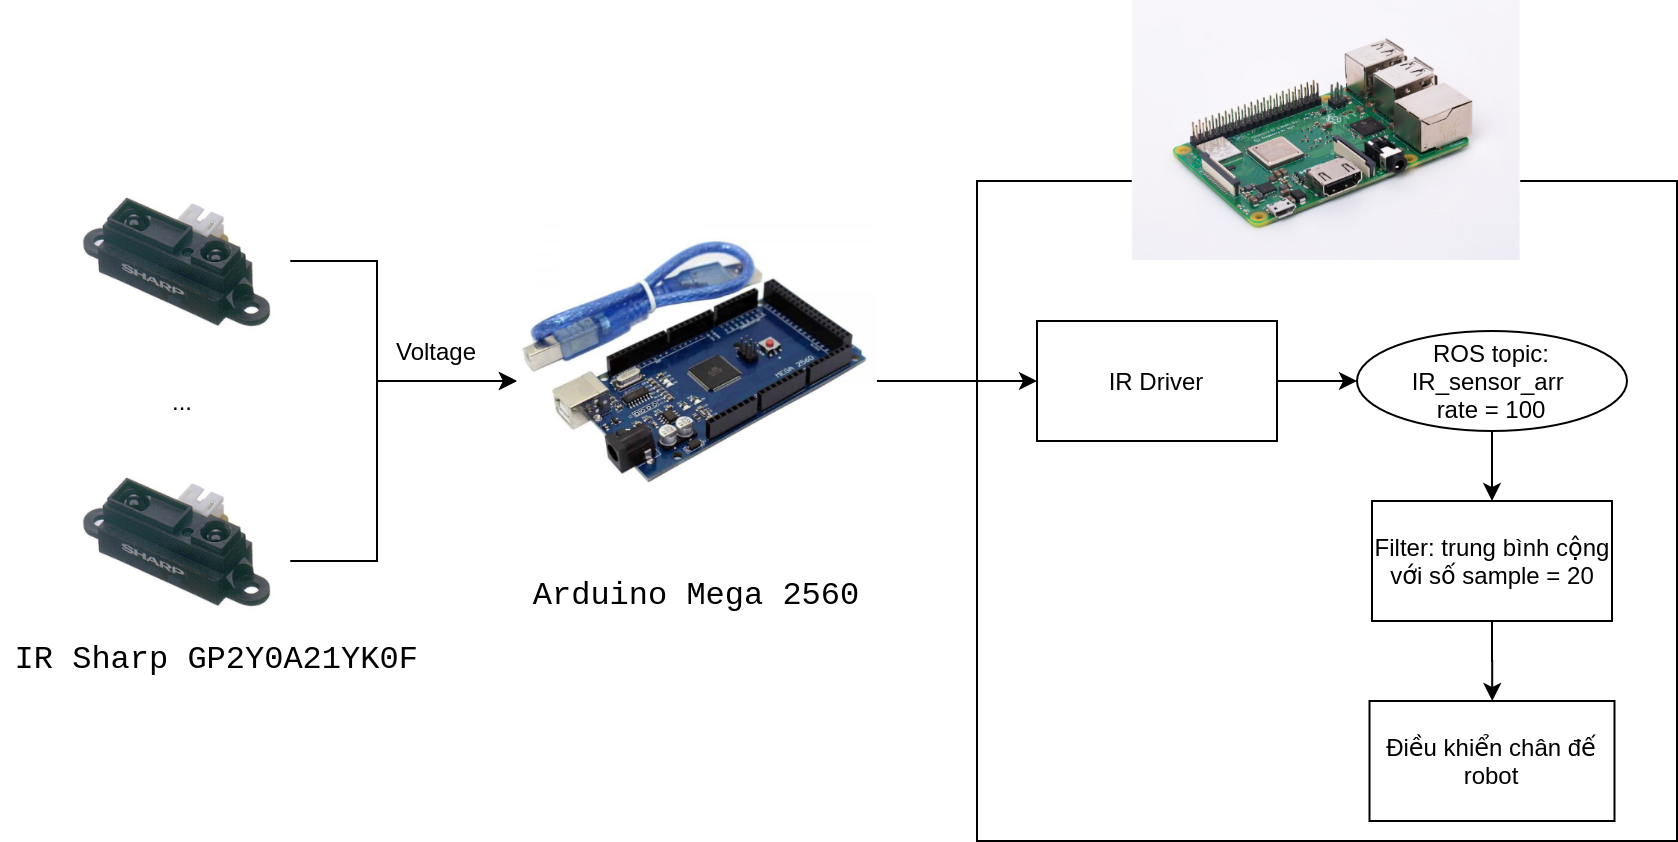
\includegraphics[width=\linewidth]{figures/ir_safety_controller-dataProcessing.png}
    \caption{Sơ đồ xử lý dữ liệu cảm biến}
    \label{fig:workflow-dataProcessing}
\end{figure}

Mạch Arduino Mega sẽ đọc tín hiệu điện trả về từ các cảm biến IR mỗi khi có lệnh yêu cầu từ Raspberry Pi. Mỗi chân dữ liệu của cảm biến kết nối với chân Analog input trên mạch Arduino để đọc dữ liệu điện áp thông qua ADC 8 bit.
Trên Raspberry Pi, {\tt node ir\_driver} sẽ nhận các dữ liệu ADC của các cảm biến từ Arduino. \figurename{ \ref{fig:irSharp-vol-distance}} cho ta mối liên hệ giữa điện áp và khoảng cách của cảm biến SHARP GP2Y0A21YK0F. Tuy nhiên, đây là đồ thị một đường cong không được biểu diễn bởi một hàm toán học cụ thể. Phương pháp được sử dụng là dùng thí nghiệm đo với giá trị điện áp và khoảng cách tương ứng. Sau đó nội suy kết quả thí nghiệm thành một hàm toán học gần đúng. Trong luận văn này, sử dụng công thức \ref{equa:ADC2Vol} và \ref{equa:Vol2Distance} \footnote{\url{https://github.com/guillaume-rico/SharpIR}} và kiểm nghiệm thấy kết quả khá chính xác (tại \ref{sub:DanhgiaCBIR})

\begin{equation}
    v = \frac{ADC * 5.0}{1023.0}
    \label{equa:ADC2Vol}
\end{equation}

\begin{equation}
    d = 27.728 * {v}^{-1.2045}
    \label{equa:Vol2Distance}
\end{equation}

Trong đó:
\begin{itemize}
    \item v - Điện áp ghi nhận tại chân analog của arduino.
    \item d - Khoảng cách đo được từ cảm biến
\end{itemize}

Sau khi tính được khoảng cách của các cảm biến sẽ {\tt publish} ra {\tt topic IR\_sensor\_arr} chứa thông tin đo được từ tất cả các cảm biến với tần số 20Hz.
%FIXME: Hiện tại trong chương trình đang để tần số 100Hz, tuy nhiên xem lại data sheet thì tần số đo của cảm biến này chỉ đạt 26Hz.

\begin{equation}
    d = \frac{\sum_{i=1}^{N} d_i}{N}
    \label{equa:Med_filter}
\end{equation}

Sau đó dùng bộ lọc trung bình cộng để lấy trung bình cộng \ref{equa:Med_filter} của N lần đo để giảm tác động của nhiễu. Để đảm bảo hệ thống vừa hoạt động được theo thời gian thực và vừa đảm bảo độ chính xác, tin cậy, tác giả chọn N = 10 với tần số cập nhật 2 lần/giây (Chi tiết tại mục \ref{sub:DanhgiaCBIR})

\subsection{Trình bày giải thuật} \label{sub:IR-algorithm}
%TODO: Trình bày giải thuật điều khiển 2 mức: bubble boudary bên ngoài và vòng tròn nguy cấp bên trong. Tuy nhiên phần này chưa điều chỉnh thông số thuật toán nên

\begin{figure}[htbp]
    \centering
    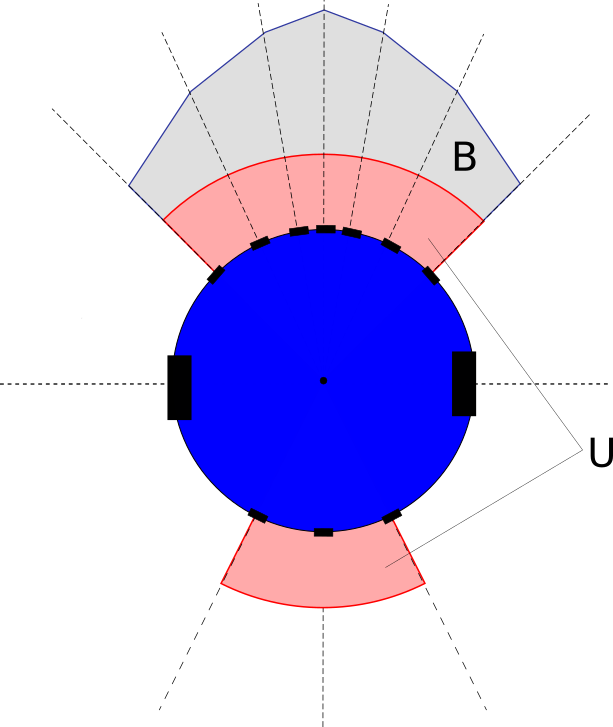
\includegraphics[width=0.5\linewidth]{figures/arg_obstacle-detection-area.png}
    \caption{Vùng xác định vật cản}
    \label{fig:arg-obstacle-area}
\end{figure}

Tác giả đề xuất sử dụng phối hợp hai giải thuật để điều khiển robot tránh vật cản sử dụng tầng cảm biến hồng ngoại. Định nghĩa hai vùng phát hiện vật cản. Vùng B và vùng U như \figurename{ \ref{fig:arg-obstacle-area}}. Chúng ta đặt mức độ ưu tiên khác nhau cho từng vùng, với mức ưu tiên áp dụng giải thuật vùng U cao hơn vùng B. Chi tiết giải thuật được mô tả như sau:

\textbf{Vùng khẩn cấp U}:
Vùng này thể hiện vùng nguy hiểm, được xác định bằng một đường tròn bán kính ${R}_{U}$ từ tâm của robot. Khi phát hiện có vật cản nằm trong vùng này nếu robot có lệnh di chuyển tiến hoặc lùi thì sẽ dừng lại, di chuyển robot lùi/tiến để tránh khỏi vật cản, đồng thời phát âm thanh để thông báo có vật cản cho đến khi không còn vật cản trong vùng này.
\begin{figure}[]
    \centering
    \begin{tikzpicture}[node distance=2cm]
        % \node (start) [startstop] {Bắt đầu};
        \node (in1) [io] {Lấy dữ liệu cảm biến ${IR}_{i}$};
        \node (dec1) [decision, below of=in1] {${IR}_{i} < {R}_{U}$};
        \node (dec2) [decision, below of=dec1, aspect=2, node distance=4cm, xshift = -3cm] {$i = [0..7]$ và $v > 0$};
        \node (dec3) [decision, below of=dec1, aspect=2, node distance=4cm, xshift = 3cm] {$i = [8..10]$ và $v < 0$};
        % \node (dec4) [decision,text width=3.5cm, aspect=1.5, below of=dec1, node distance=3cm, xshift=5.5cm] {$i = [8..10]$ và $i = [0..7]$ và $v \neq 0$};
        \node (proc1) [process, below of=dec2, node distance=3cm,xshift = 0cm] {Lùi + Phát âm thanh};
        \node (proc2) [process, below of=dec3, node distance=3cm,xshift = 0cm] {Tiến + Phát âm thanh};

        % \draw [arrow] (start) -- (in1);
        \draw [arrow] (in1) --  (dec1);
        \draw [arrow] (dec1) -- (0,-3.5) -| (dec2);
        \draw [arrow] (dec2) -- node[anchor=east] {Đúng}(proc1);
        \draw [arrow] (dec2) --++ (-3,0) |- node[anchor=east] {Sai} (in1);
        \draw [arrow] (dec3) -- node[anchor=east] {Đúng}(proc2);
        \draw [arrow] (dec3) --++ (3,0) |- node[anchor=west] {Sai} (in1);
        % \draw [arrow] (dec2) -- node[anchor=east] {Sai}(dec3);
        \draw [arrow] (dec1) -- node[anchor=east] {Đúng}(0,-3.5) -| (dec3);
    \end{tikzpicture}
    \caption{Sơ đồ giải thuật vùng khẩn cấp U}
    \label{flowchart-urgent}
\end{figure}

\begin{figure}[htbp]
    \centering
    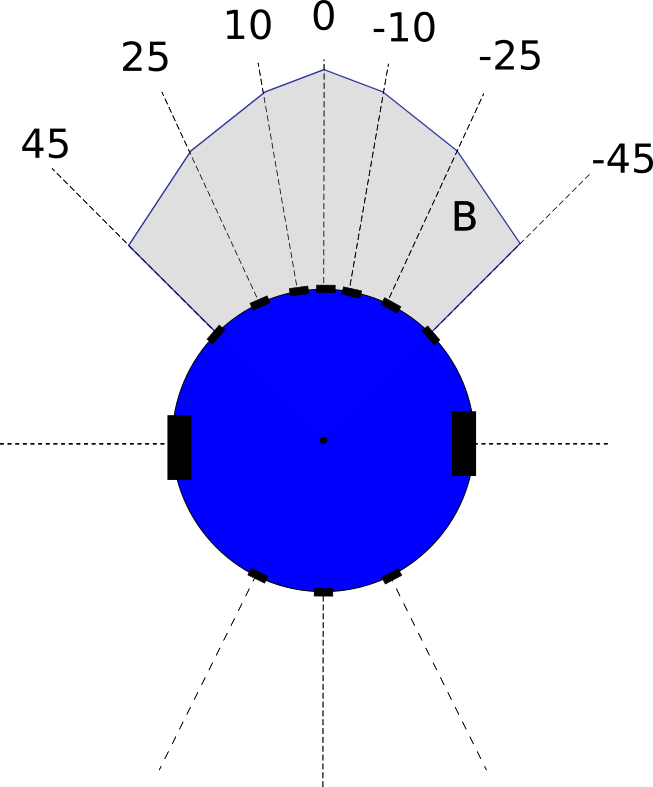
\includegraphics[width=0.4\linewidth]{figures/BB-argorithm.png}
    \caption{Hình dạng bong bóng phản ứng}
    \label{fig:BB-argorithm}
\end{figure}

\begin{figure}[htbp]
    \centering
    \subfloat[]{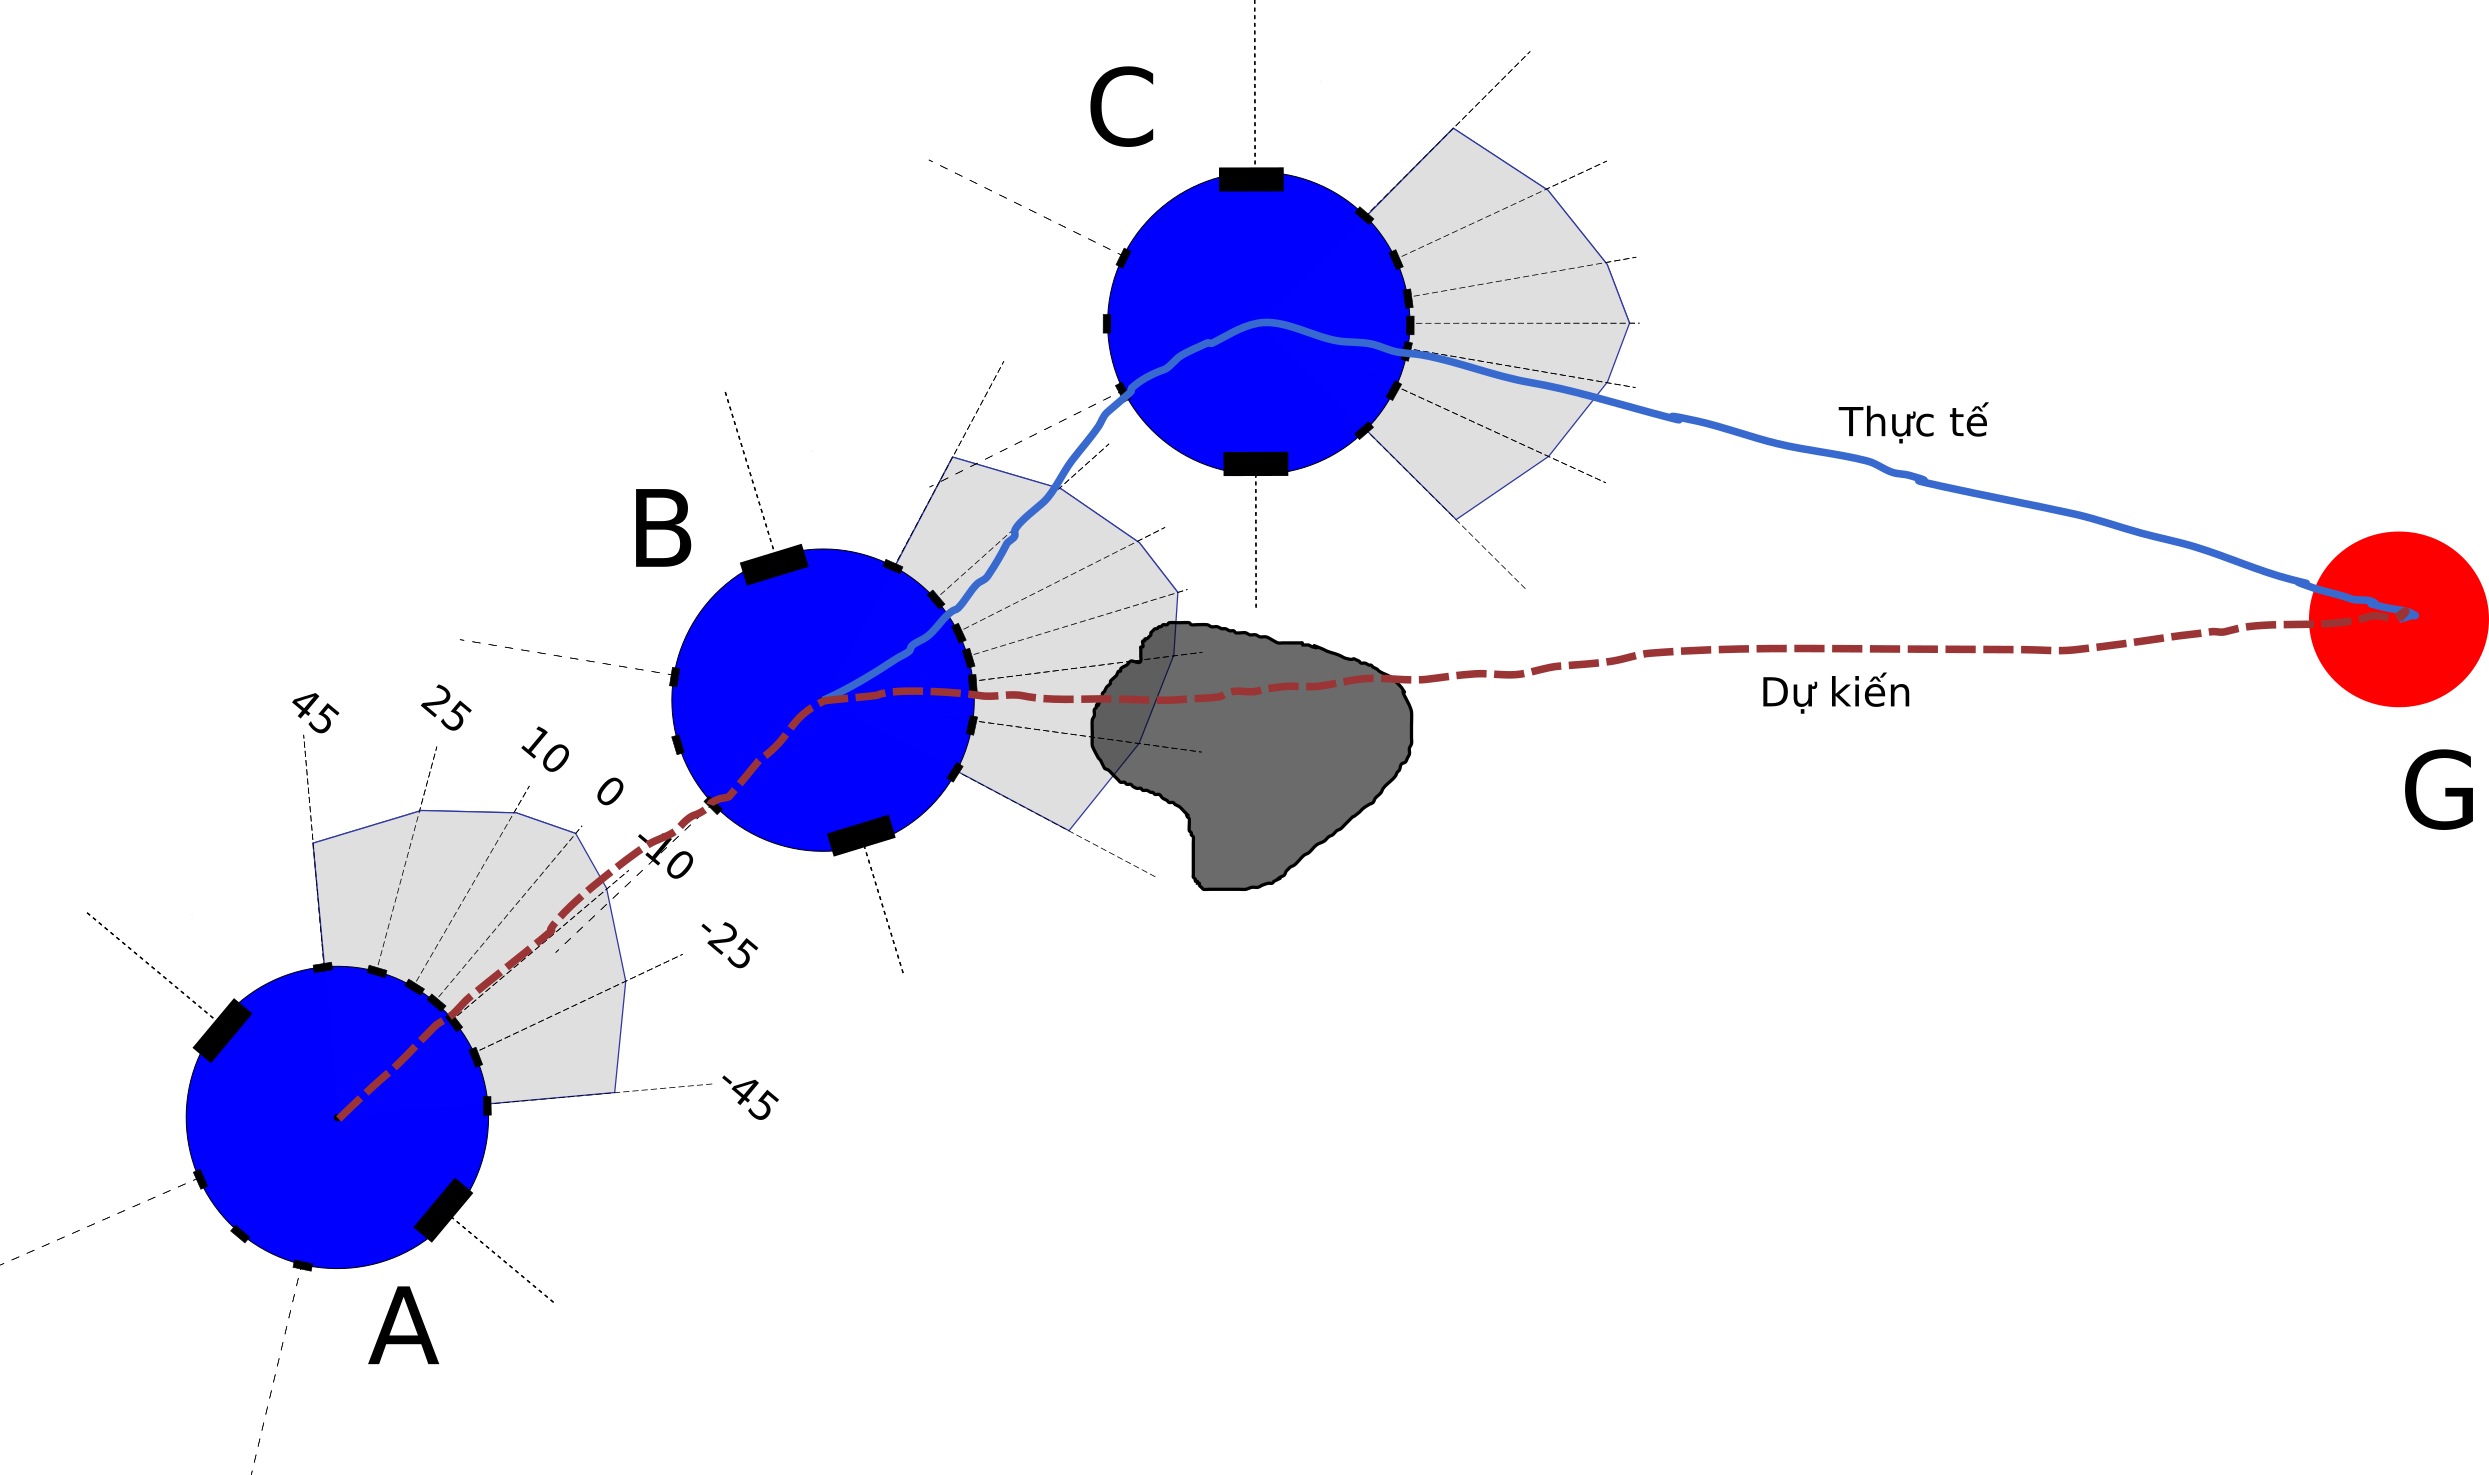
\includegraphics[width=0.75\linewidth]{figures/IR_BB-avoidance.png}} \\
    \subfloat[]{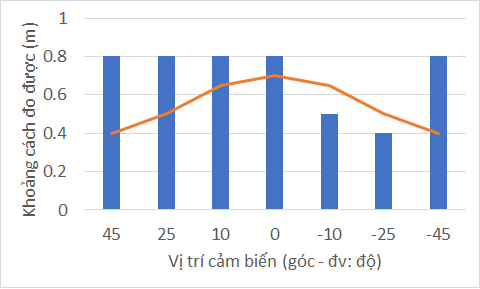
\includegraphics[width=0.5\linewidth]{figures/BB_chart.png}}
    \caption{Giải thuật tránh vật cản bằng bong bóng phản ứng}
    \label{fig:BB-avoidance}
\end{figure}

\textbf{Bong bóng phản ứng B}:
Trên cơ sở tham khảo \cite{Susnea2009}, thuật toán bong bóng phản ứng xác định một đường bao phía trước robot, có hình dạng như trong Hình \ref{fig:BB-argorithm}, kích thước đường bao được làm mới sau mỗi chu kì ${\Delta}{t}$, phụ thuộc vào vị trí cảm biến và vận tốc di chuyển của robot theo công thức \ref{equa:BB-update}. Trong đó $bb[i]$ là kích thước bong bóng tại vị trí cảm biến thứ i, $K_i$ là hệ số, $V_t$ là vận tốc dài của robot tại thời điểm t, $\Delta_t$ là khoảng thời gian giữa 2 lần cập nhật.
Kích thước đường bao là phạm vi đảm bảo robot có thể di chuyển tự do trong khoảng thời gian $\Delta_t$ mà không va chạm với vật cản.

\begin{equation}
    bb[i] = K_i*V_t*\Delta_t
    \label{equa:BB-update}
\end{equation}

\figurename{ \ref{fig:BB-avoidance}}a mô tả một trường hợp hoạt động của thuật toán tránh vật cản bằng thuật toán bong bóng phản ứng. Robot di chuyển từ vị trí A tới đích G với quỹ đạo được chương trình \codeword{slam_gmapping} tính toán theo đường nét đứt. Tuy nhiên, đến vị trí B, robot phát hiện thấy vật cản mà Lidar không phát hiện ra được. Giá trị đo được của cảm biến và giá trị bong bóng phản ứng tại điểm B được mô tả trong biểu đồ Hình \ref{fig:BB-avoidance}b. Có hai cảm biến tại vị trí góc -10 và -25 có khoảng cách đo được nhỏ hơn giá trị của bong bóng phản ứng, do đó đánh dấu 2 vị trí này có vật cản. Robot xác định có xuất hiện vật cản tại phía trước, bên phải, do đó, chân đế của robot được ra lệnh giảm vận tốc và đồng thời quay trái. Vì vị trí và hướng của robot lúc này đã lệch khỏi đường đi dự kiến ban đầu, do đó chương trình \codeword{slam_gmapping} tính toán lại quỹ đạo mới di chuyển tới đích, là đường nét liền màu xanh.
% trí gặp vật cản robot thực hiện quay mình để tránh vật cản, sau đó phần điều hướng trong robot lại tính lại đường đi tới đích (đường màu xanh).

\section{Phối hợp điều khiển robot}
\subsection{Tích hợp vào bản đồ địa phương}

Hệ thống điều khiển di chuyển cho robot bao gồm hai gói chương trình chính là \codeword{dashgo_driver} chứa các chương trình điều khiển chân đế di chuyển và \codeword{dashgo_nav} chứa các chương trình tạo bản đồ, tính toán quỹ đạo di chuyển... Chi tiết về điều khiển di chuyển robot được trình bày trong mục \ref{sub:software-architecture}.
Trong phần này, sau khi phát triển xong hệ thống phát hiện và điều khiển tránh vật cản bằng cảm biến hồng ngoại, tác giả sẽ tích hợp vào trong hệ thống điều khiển robot. Các dữ liệu từ cảm biến hồng ngoại khi phát hiện vật sẽ được đánh dấu vào trong bản đồ giá trị địa phương. Đồng thời khi vật cản nằm trong vùng bong bóng phản ứng B hoặc vùng khẩn cấp U, chương trình điều khiển sẽ điều khiển theo thuật toán được trình bày trong \ref{sub:IR-algorithm}. Vì vậy, sau khi phản ứng với vật cản, trên bản đồ đã cập nhật vị trí của vật cản nên chương trinh tạo quỹ đạo mới sẽ đưa robot tránh khỏi vật cản được phát hiện bởi hệ thống cảm biến hồng ngoại.

\subsection{Phân quyền điều khiển}
Trong một vài trường hợp, có thể có nhiều chương trình, nhiều thuật toán được sử dụng để thực hiện cùng một tác vụ nào đó. Trong robot tự hành Dashgo D1, có nhiều chương trình khác nhau có thể tác động đến việc di chuyển của nó. Ví dụ trong phần lớn thời gian robot di chuyển dưới sự điều khiển của chương trình \codeword{slam_navigation}, khi có tín hiệu điều khiển bằng tay từ bàn phím, robot lại chạy dưới sự điều khiển của chương trình \codeword{teleop}, khi gặp vật cản được phát hiện bởi cảm biến sonar, robot phản ứng dừng lại hoặc quay trái/phải để tránh vật cản. Như trường hợp đơn giản vừa rồi có tới ba tiến trình cùng đồng thời điều khiển robot.

\begin{figure}[htbp]
    \centering
    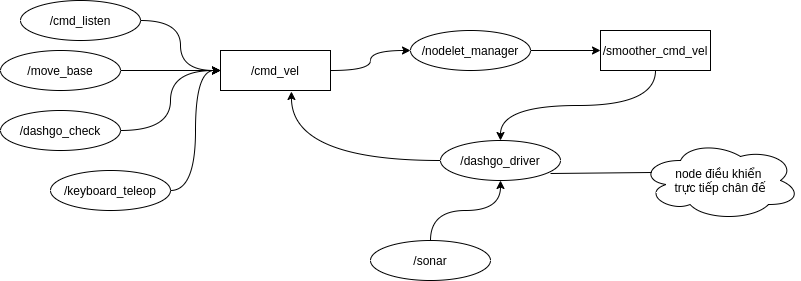
\includegraphics[width=\linewidth]{figures/phanquyen-goc.png}
    \caption{Sơ đồ điều khiển chân để robot}
    \label{fig:phanquyen-goc}
\end{figure}

\figurename{ \ref{fig:phanquyen-goc}} thể hiện các node và topic điều khiển robot Dashgo D1. Trong đó, topic \codeword{/cmd_vel} nhận thông tin điều khiển di chuyển chân đế từ nhiều topic khác nhau. Sau đó thông qua trình quản lý \codeword{nodelet_manager} để chạy chương trình làm mịn tốc độ, chống giật cho robot. \codeword{/smoother_cmd_vel} được topic \codeword{/dashgo_driver} nhận và thực hiện các tính toán điều khiển tới vòng quay của động cơ để di chuyển.
Ta thấy có \codeword{/sonar} được liên kết trực tiếp với \codeword{/dashgo_driver}, ở robot này, dữ liệu từ các cảm biến siêu âm được driver điều khiển chân đế đọc trực tiếp, sau đó xử lý các tình huống và tính toán số vòng quay của động cơ để thực hiện điều khiển chân đế trong trường hợp khẩn cấp.

% \subsection{Phương pháp phối hợp phân mức điều khiển}

\begin{figure}[htbp]
    \centering
    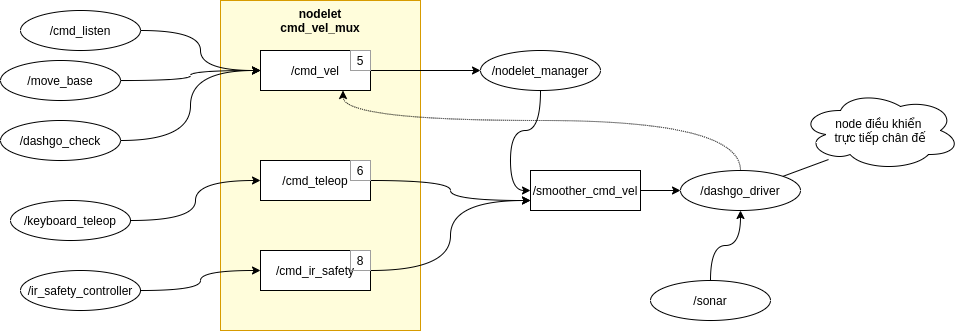
\includegraphics[width=\linewidth]{figures/phanquen-dexuat.png}
    \caption{Thiết kế phân quyền điều khiển}
    \label{fig:phanquen-dexuat}
\end{figure}

Có một vài phương pháp để phối hợp phân quyền điều khiển cho robot. Khi chúng ta có nhiều thuật toán, nhiều chương trình cùng điều khiển tới một hoạt động nào đó.
% ROS có định nghĩa \codeword{nodelet}\footnote{\url{http://wiki.ros.org/nodelet}}.
Trong luận văn này, tác giả sử dụng \codeword{cmd_vel_mux} của \codeword{nodelet} để thực hiện phân quyền điều khiển cho robot để dễ dàng tích hợp tín hiệu điều khiển từ cảm biến an toàn IR (Hình \ref{fig:phanquen-dexuat})

%=======================================
% \section{Đánh giá hệ thống tránh vật cản}}
\section{Kết quả và đánh giá}
\label{sec:testbed}

%---
% - Tiến hành thí nghiệm, nêu rõ bài toán thí nghiệm
% - Đánh giá kết quả (Hiệu quả hay không, vì sao)
%---

\subsection{Kết quả của luận văn}

Sau quá trình nghiên cứu và làm việc, tác giả đã có một số kết quả như sau:
\begin{itemize}
    \item Làm chủ hệ thống điều khiển robot, tạo bản đồ và di chuyển trong bản đồ.
    \item Phát triển hệ thống phần cứng robot. Hình \ref{fig:RB-multi-sensor-layer} là kết quả sau khi lắp hệ thống lên robot, robot có thể phát hiện và tránh vật cản bằng 3 tầng cảm biến siêu âm, lidar và hồng ngoại.
    \item Đề xuất và thử nghiệm hệ thống tránh vật cản bằng cảm biến đa tầng, bao gồm bố trí cảm biến, xử lý tín hiệu đo, giải thuật điều khiển.
    \item Nghiên cứu xây dựng hệ thống điều khiển phân quyền nhiều mức ưu tiên cho robot.
\end{itemize}

\begin{figure}[htbp]
    \centering
    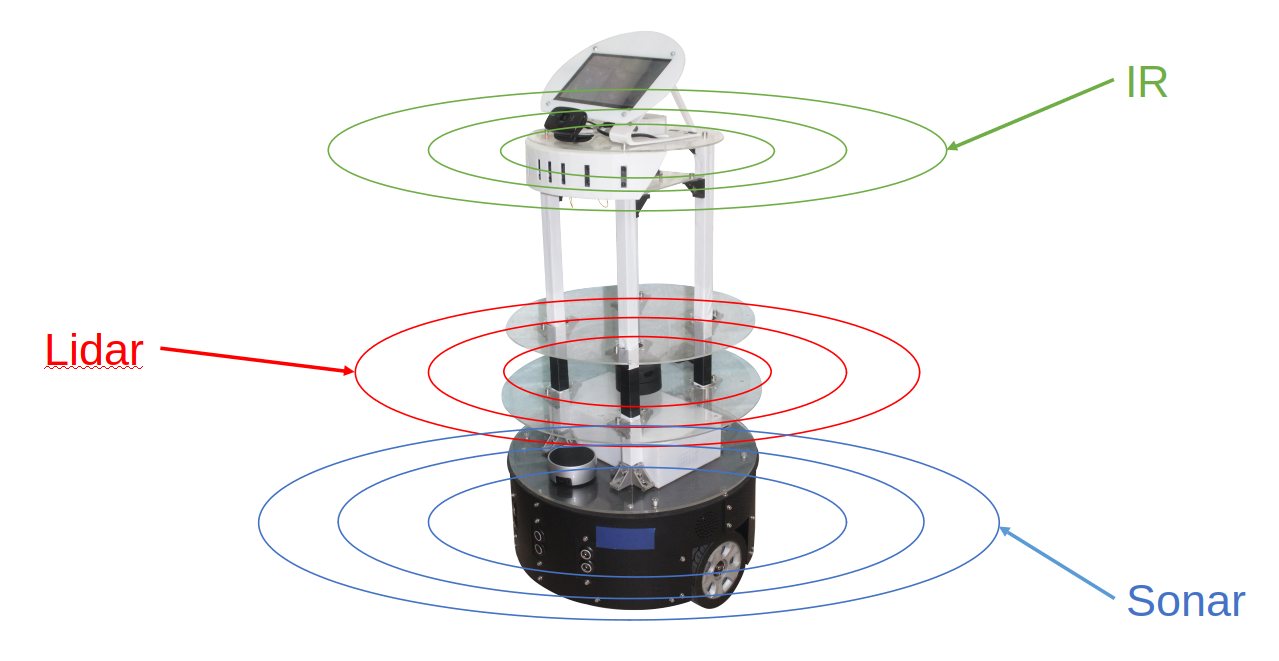
\includegraphics[width=0.75\linewidth]{figures/rb_Multi_Sensor_layer.png}
    \caption{Ba tầng cảm biến phát hiện vật cản trên robot}
    \label{fig:RB-multi-sensor-layer}
\end{figure}

\subsection{Đánh giá độ chính xác cảm biến khoảng cách hồng ngoại}
\label{sub:DanhgiaCBIR}
%------------------------------------------

Thực hiện đánh giá độ chính xác của cảm biến khoảng cách hồng ngoại IR Sharp GP2Y0A21YK0F. Tác giả bố trí thí nghiệm đo trên từng cảm biến riêng lẻ. Kết quả đo tại 8 vị trí khoảng cách 0.1m, 0.2m, 0.3m, 0.4m, 0.5m, 0.6m, 0.7m, 0.8m với 100 lần lấy mẫu, tần số lấy mẫu là 20Hz được kết quả đo như biểu đồ Hình \ref{fig:Ir-eval-100}.

\begin{figure}[htbp]
    \centering
    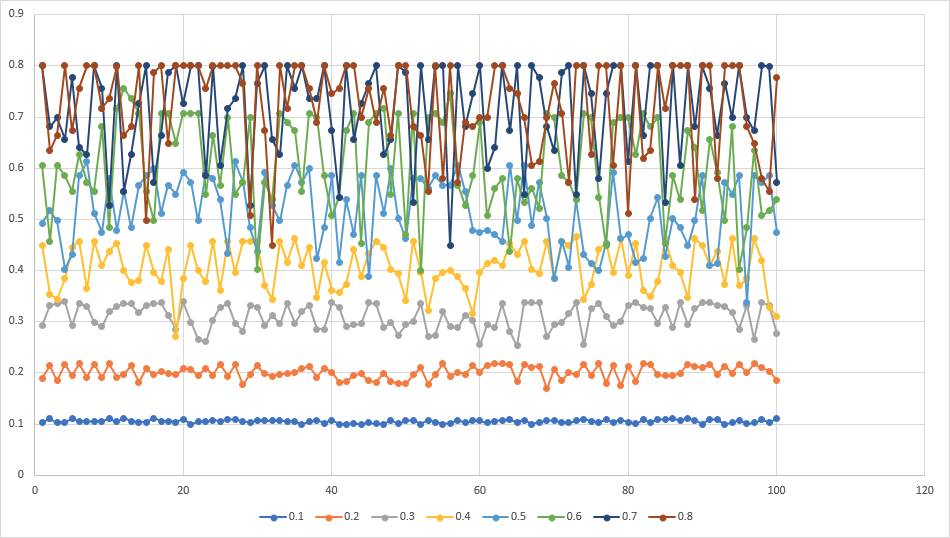
\includegraphics[width=\linewidth]{figures/IR-eval-chart.png}
    \caption{Kết quả đo cảm biến}
    \label{fig:Ir-eval-100}
\end{figure}

\begin{table}[htbp]
    \begin{tabular}{|m{1.5cm}|m{1.2cm}|m{1.2cm}|m{1.2cm}|m{1.2cm}|m{1.2cm}|m{1.2cm}|m{1.2cm}|m{1.4cm}|}
        \hline
        Cần đo     & 0.1      & 0.2      & 0.3      & 0.4      & 0.5      & 0.6      & 0.7      & 0.8      \\ \hline
        Trung bình & 0.1051   & 0.2009   & 0.3100   & 0.4068   & 0.5157   & 0.6086   & 0.7146       & 0.7229 \\ \hline
        Sai số tb & 0.0051 & 0.0009 &   0.0100 & 0.0068 &   0.0157 & 0.0086 &   0.0146 & -0.0771 \\ \hline
        \% sai số  & 5.14\% & 	0.44\% &	3.34\% &	1.69\% &	3.14\% &	1.43\% &	2.08\% &	9.63\% \\
        \hline
    \end{tabular}
    \caption{Giá trị đo trung bình 100 mẫu}
    \label{table:ir-evarage}
\end{table}


\begin{figure}[htbp]
    \centering
    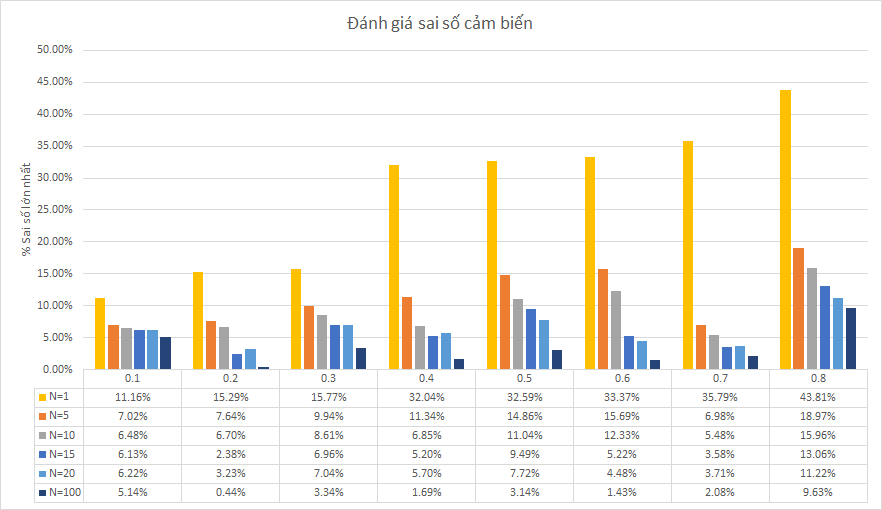
\includegraphics[width=\textwidth]{figures/chart_IReval_MaxPercent.png}
    \caption[Đánh giá sai số lớn nhất tương ứng với số lần lấy mẫu]{Đánh giá sai số lớn nhất tương ứng với số lần lấy mẫu trên một lần đo N = 1, 5, 10, 15, 20 và 100}
    \label{chart:IR-eval-NumSample}
\end{figure}

 Giá trị trung bình của 100 lần đo và sai số được thể hiện trong Bảng \ref{table:ir-evarage}. Từ đây ta thấy với trung bình của 100 lần đo thì sai số nằm trong giới hạn sai số cho phép 5\% với phép đo trong khoảng 0.1-0.7m.
%  Do cảm biến IR Sharp GP2Y0A21YK0F có khoảng đo từ 10 - 80 cm nên tác giả đã đặt khoảng cách đo giới hạn từ 10 - 80 cm. Do đó trong biểu đồ Hình \ref{fig:Ir-eval-100} kết quả đo bị chặn dưới tại 0.1m và chặn trên tại 0.8m.
%  Hình \ref{fig:IR-evel-N1} thể hiện sai số trong phép đo cảm biến.

\begin{figure}[htbp]
\centering
\subfloat[][]{
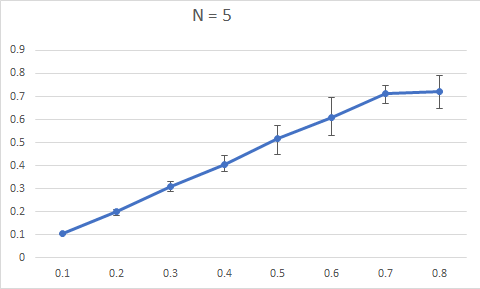
\includegraphics[width = 0.45 \linewidth]{figures/chart_IReval_N5.png}
}
\subfloat[][]{
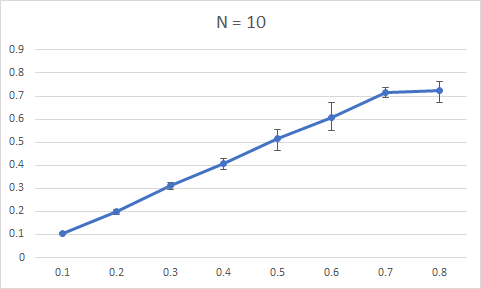
\includegraphics[width = 0.45 \linewidth]{figures/chart_IReval_N10.png}
}
\hspace{8pt}
\subfloat[][]{
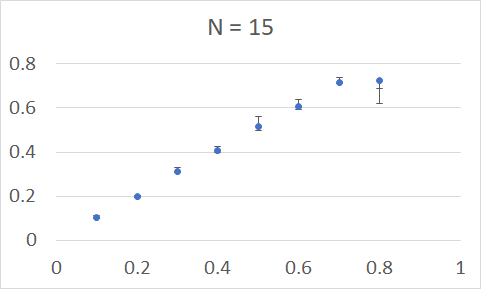
\includegraphics[width = 0.45 \linewidth]{figures/chart_IReval_N15.png}
}
\subfloat[][]{
    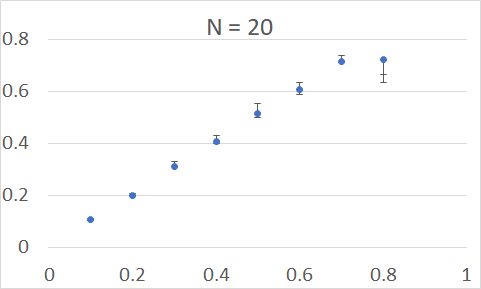
\includegraphics[width = 0.45 \linewidth]{figures/chart_IReval_N20.png}
    }
    \caption{Sai số tương ứng với N lần lấy mẫu}
    \label{fig:chart-IR-N-errorbar}
\end{figure}

Tác giả áp dụng bộ lọc trung bình cộng (công thức \ref{equa:Med_filter}) để giảm nhiễu và sai số trong kết quả đo. Tuy nhiên, trong thực tế, robot di chuyển theo thời gian thực, do đó số lần lấy mẫu cho một lần đo N bị giới hạn. Biểu đồ Hình \ref{chart:IR-eval-NumSample} đánh giá sai số lớn nhất với các giá trị N khác nhau. Hình \ref{fig:chart-IR-N-errorbar} thể hiện mức độ hội tụ của kết quả đo tương ứng với các giá trị N khác nhau. Qua đây chúng ta có thể thấy khi tăng N thì sai số trong phép đo càng giảm và giá trị đo càng hội tụ. Tuy nhiên, để đảm bảo robot cập nhật kết quả đo theo thời gian thực, tác giả chọn N = 10 tương ứng với tần số cập nhật kết quả đo là 2 lần/giây.

%============================================================
\subsection{Đánh giá giải thuật điều khiển tích hợp cảm biến}
%------------------------------------------------------------
% \subsubsection*{Phương pháp đánh giá}
% \subsubsection*{Kết quả đạt được}
% \subsubsection*{Robot phản ứng với vật cản tĩnh}

Ưu điểm của hệ thống tránh vật cản bằng phối hợp nhiều tầng cảm biến là robot có thể di chuyển an toàn được trong các môi trường với đa dạng đối tượng hơn như bàn, ghế, các đối tượng mà bài toán định vị dẫn đường 2D chỉ với một tầng cảm biến có thể không đáp ứng được khi vật cản không nằm trong mặt phẳng quét của LIDAR.

\begin{figure}[htbp]
    \centering
    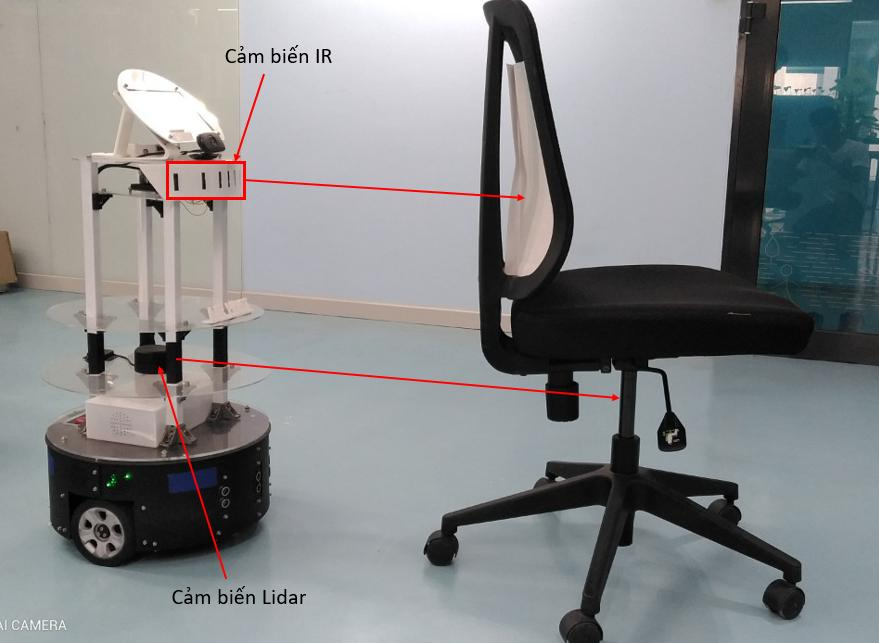
\includegraphics[width=0.75\linewidth]{figures/RB_scenario_ir_detectingObstacle.png}
    \caption{Robot với vật cản có biên dạng biến đổi theo chiều cao}
    \label{fig:scenario_ir_detectedObstacle}
\end{figure}

\begin{figure}[htbp]
    \centering
    \subfloat[]{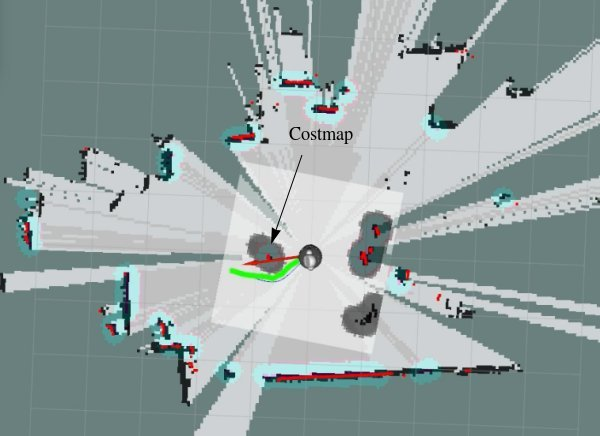
\includegraphics[width=0.75\linewidth]{figures/RB_navi_without_IR.jpg}}
    \hspace{8pt}
    \subfloat[]{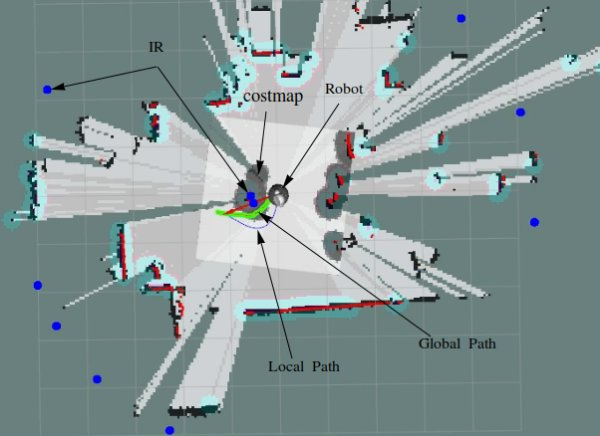
\includegraphics[width=0.75\linewidth]{figures/RB_navi_with_IR.jpg}}
    \caption{Bản đồ thể robot phát hiện ghế xoay khi không có hệ thống cảm biến hồng ngoại (Hình a) và khi có hệ thống hồng ngoại (Hình b)}
    \label{fig:rb_with_obstacle_in_rviz}
\end{figure}

% \begin{figure}[htbp]
%     \centering
%     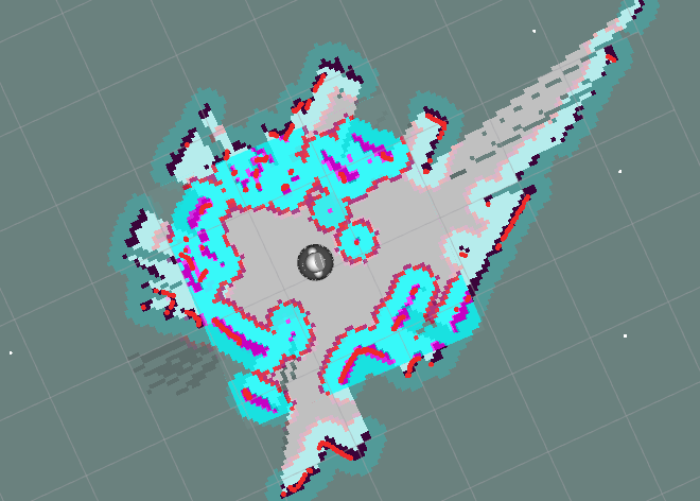
\includegraphics[width=0.75\linewidth]{figures/RB_withoutIR_obstacleDetect.png}
%     \caption{Trường hợp không kích hoạt lớp tránh vật cản bằng hồng ngoại}
%     \label{fig:rb_withoutIR}
% \end{figure}

Hệ thống phát hiện và tránh được vật cản, đồng thời phối hợp với hai tầng cảm biến sẵn có trên robot là cảm biến LIDAR và cảm biến tránh vật cản bằng siêu âm. Khi xuất hiện vật cản, robot sẽ tránh theo giải thuật được mô tả tại mục \ref{sec:caitienhethongtranhvatcan} và đồng thời đánh dấu vật cản vào bản đồ cục bộ để giúp robot tạo đường đi mới mà không lặp lại đường cũ.

Hình \ref{fig:scenario_ir_detectedObstacle} thể hiện một trường hợp robot đối diện với vật cản có hình dạng biến đối theo chiều cao, là ghế xoay. Đối với ghế xoay, tầng cảm biến Lidar của robot quét được vùng chỉ có trụ chống của ghế. Vì vậy với cảm biến Lidar, robot thấy ghế xoay chỉ là một vật thể rất nhỏ. Hình \ref{fig:rb_with_obstacle_in_rviz}a thể hiện trên bản đồ khi chỉ có tầng Lidar, ghế xoay được đánh dấu bằng một chấm nhỏ và khi di chuyển tới điểm đích phía trước thì robot sẽ va chạm với ghế. Khi có hệ thống cảm biến hồng ngoại tránh vật cản ở tầng cao của robot, robot sẽ phát hiện ra phía tựa lưng của ghế và đánh dấu vào bản đồ một diện tích chiếm dụng nhiều hơn (Hình \ref{fig:rb_with_obstacle_in_rviz}b). Do đó, khi cho di chuyển tới một điểm đích phía trước ghế, robot sẽ tạo đường đi tránh ra khỏi vùng được đánh dấu và không bị va chạm với ghế.

Phần vật cản được đánh dấu vào bản đồ bởi cảm biến hồng ngoại không được ghi nhận vào bản đồ như một vật cố định mà được coi là một vật cản mới xuất hiện trong bản đồ. Trong Hình \ref{fig:rb_with_obstacle_in_rviz}b, chúng ta thấy đường đi toàn cục (\textit{Global Path}) đi qua phần bị đánh dấu màu xám, đây là đường đi được tính trên toàn cục dựa trên bản đồ. Tuy nhiên, đường đi thực tế của robot là theo đường đi cục bộ (\textit{Local Path}) được xác định dựa dựa trên bản đồ giá trị cục bộ (\textit{Local costmap})
%Tuy nhiên, với hệ thống mới mà tác giả đề xuất, robot có thể phát hiện được phần biên dạng phía trên của đối tượng và đánh dấu là vật cản trong bản đồ Hình \ref{fig:rb_withIR_ObstacleDetected}. Do đó, khi cho robot di chuyển tới vị trí phía sau đối tượng, robot tạo đường đi tránh vật cản và di chuyển vòng qua nó như trong Hình \ref{fig:rb_withIR_ObstacleDetected}b.

\begin{figure}[htbp]
    \centering
    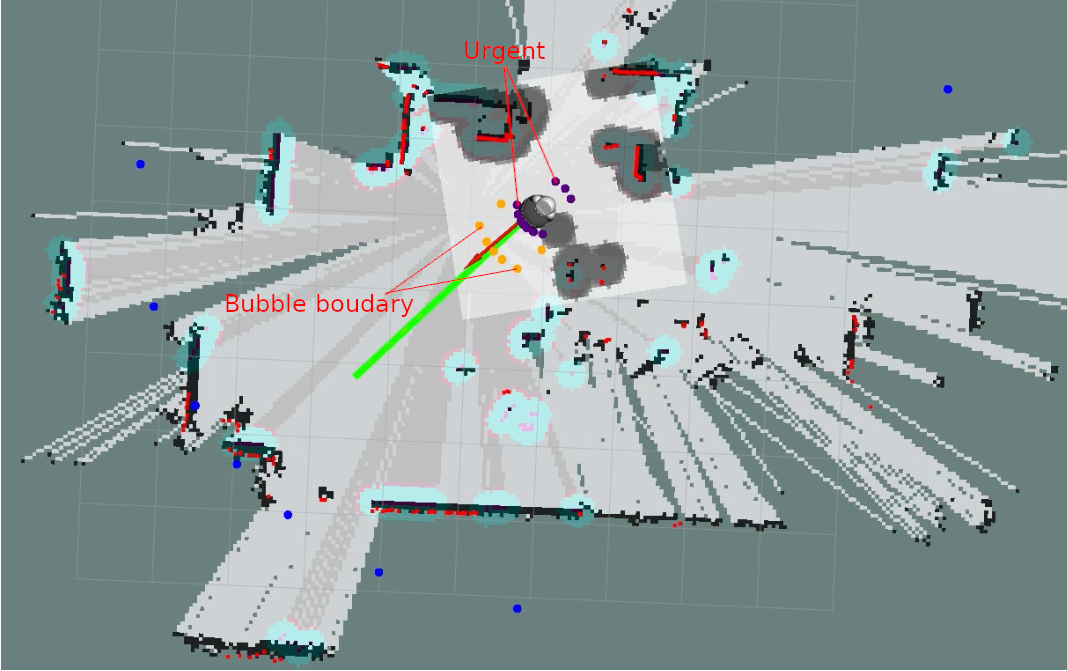
\includegraphics[width=0.9\linewidth]{figures/RB_bb_urgent.png}
    \caption{Vùng khẩn cấp U và bong bóng phản ứng B trong quá trình di chuyển của robot}
    \label{fig:bb_urgent}
\end{figure}

\begin{figure}[htbp]
    \centering
    \subfloat[]{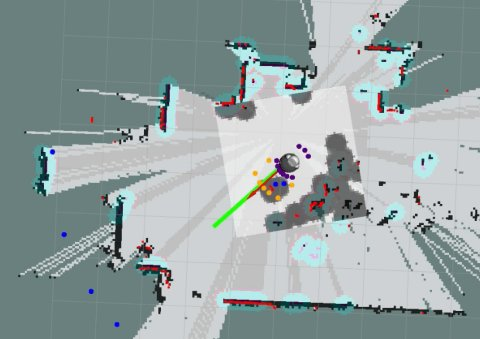
\includegraphics[width=0.6\linewidth]{figures/RB_bb_detect_obstacle.jpg}}
    \hspace{8pt}
    \subfloat[]{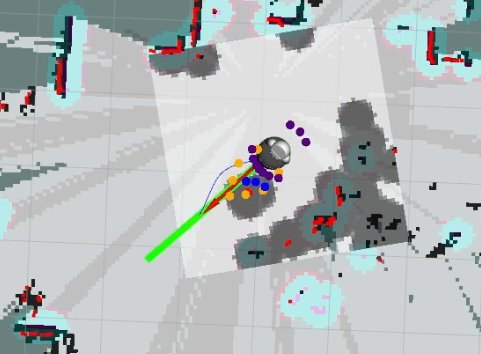
\includegraphics[width=0.6\linewidth]{figures/RB_bb_detect_obstacle_reAct.jpg}}
    % \qquad
    \hspace{8pt}
    \subfloat[]{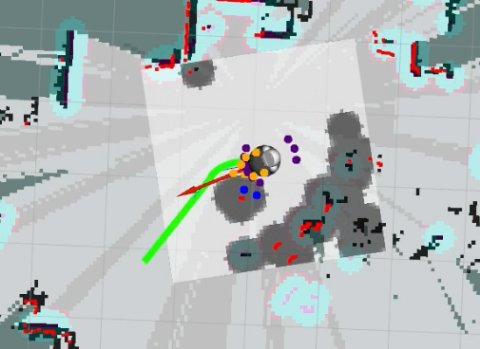
\includegraphics[width=0.6\linewidth]{figures/RB_bb_detect_obstacle_avoided.jpg}}
    \caption{Robot phản ứng với vật cản động}
    \label{fig:ir-detected-reaction}
\end{figure}

Hình \ref{fig:bb_urgent} thể hiện giới hạn vùng khẩn cấp U và bong bóng phản ứng B trong quá trình di chuyển của robot. Trường hợp vật cản xuất hiện với tốc độ nhanh\footnote{Chưa có đánh giá nhanh như thế nào}. Trong hình \ref{fig:ir-detected-reaction}a, vật cản xuất hiện và hệ thống cảm biến hồng ngoại phát hiện có vật cản trong vùng bong bóng phản ứng ở phía trước, bên trái robot. Lúc này, chương trình điều khiển tránh vật cản bằng hệ cảm biến hồng ngoại giành lấy quyền điều khiển, thực hiện điều khiển robot giảm tốc độ, quay sang phải, đồng thời đánh dấu vật cản vào bản đồ giá trị địa phương cũng như tính toán quỹ đạo di chuyển mới cho robot. Sau quá trình đó, robot đổi hướng di chuyển và có quỹ đạo tránh được vật cản như trong Hình \ref{fig:ir-detected-reaction}c. Qua Hình \ref{fig:ir-detected-reaction} ta cũng thấy rằng giới hạn vùng bong bóng phản ứng thay đổi theo tốc độ của robot.

Tóm lại, trong phần này, tác giả mới đánh giá được định tính về việc phát hiện và phản ứng tránh vật cản bằng cách phối hợp thêm một tầng cảm biến hồng ngoại với một số kết quả đạt được như sau:
Robot phát hiện được vật cản có hình dạng thay đổi theo chiều cao, vật cản ở tầng cao với chiều cao robot, đánh dấu vật cản vào bản đồ giá trị địa phương và phản ứng tránh vật cản từ vật cản tĩnh tới vật cản chuyển động vừa phải.

Tuy nhiên, hệ thống còn có một số điểm hạn chế như:
\begin{itemize}
    \item Hệ thống cảm biến đo chưa thực sự chính xác và ổn định, gây ra khó khăn trong quá trình áp dụng thuật toán
    \item Cảm biến hồng ngoại IR Sharp GP2Y0A21YK0F có tần số lấy mẫu tương đối thấp (tối đa 26Hz), do đó không thể tăng số lần lấy mẫu trong một lần đo, gây ảnh hưởng tới độ chính xác của kết quả đo. Bên cạnh đó, cảm biến này có khoảng đo từ 0.1-0.8m do vậy robot chỉ có thể phát hiện được vật cản trong khoảng này, điều này làm hạn chế tốc độ di chuyển có thể tránh được vật cản của robot.
\end{itemize}

% \begin{itemize}
%     \item Đánh giá cảm quan robot di chuyển và tránh được vật cản trong quá trình di chuyển ở tầng cảm biến hồng ngoại
%     \item Thực hiện thí nghiệm cho robot di chuyển giữa các điểm bất kì trong một môi trường đã được xây dựng bản đồ với các vật có hình dạng đa dạng từ thấp tới cao. Đánh giá về số lần tránh được/không tránh được vật cản
% \end{itemize}

%TODO: Bổ sung kq đánh giá thí nghiệm di chuyển

%=============================
\chapter{Kết luận và tầm nhìn}
\label{chap:KetLuan}

\section{Kết luận}
                %------------------
% Tóm tắt lại kết quả luận văn

Như vậy, sau khi làm xong luận văn này, đã đạt được một số kết quả như sau:
\begin{itemize}
    \item Làm chủ được hệ thống điều khiển robot tự hành thông minh bằng SLAM và ứng dụng hệ điều hành robot (ROS)
    \item Đề xuất phương pháp mới giúp robot tránh vật cản đa dạng hơn
    \item Đánh giá độ chính xác của cảm biến hồng ngoại, thấy rằng cảm biến hồng ngoại IR Sharp GP2Y0A21YK0F có tần số thấp, độ chính xác và ổn định ở mức vừa phải, làm hạn chế tốc độ di chuyển có thể tránh được vật cản của robot.
    \item Đề xuất hai giải thuật tránh vật cản bằng hệ thống cảm biến hồng ngoại, phối hợp được với hệ thống điều khiển robot và hai hệ cảm biến có sẵn trên robot.
    \item Đánh giá định tính hiệu quả tránh vật cản của robot sau khi có hệ thống tránh vật cản mới. Robot phản ứng như mong muốn của tác giả.
\end{itemize}

\section{Tầm nhìn}
% Hướng nghiên cứu tiếp theo
% Tối ưu hệ thống hiện tại
%------------------------
Trên Thế giới, robot tự hành thông minh đã được ứng dụng trong nhiều lĩnh vực khác nhau như đã đề cập ở \ref{sec:ungdung}. Tuy nhiên, ở Việt Nam chúng ta ứng dụng của robot tự hành thông minh rất ít, chủ yếu trong công nghiệp, hỗ trợ vận chuyển trong các nhà máy, kho hàng. Với các yêu cầu khắt khe khi đi vào thực tế. Trong thời gian tới, có một số hướng để phát triển robot tự hành thông minh như sau:
\begin{itemize}
    \item Tối ưu và tăng tính ổn định, tin cậy cho giải thuật tránh vật cản.
    \item Xây dựng chương trình để vận hành robot một cách đơn giản, hiệu quả và ổn định.
    \item Nghiên cứu và ứng dụng một số kết quả mới trong bài toán định vị và dẫn đường trong robot.
    \item Ứng dụng một số bài toán mới như xử lý ảnh ứng dụng học sâu, xử lý tiếng nói, chatbot\dots vào điều khiển robot.
\end{itemize}



%%%=======================
%%% Local Variables:
%%% mode: latex
%%% TeX-master: "../LuanVanThS_v1.0_main"
%%% End:

%----Tài liệu tham khảo-----------------------------
\bibliographystyle{ieeetr}
\bibliography{ref}
%==============================
\end{document}

%%% Local Variables:
%%% mode: latex
%%% TeX-master: t
%%% End:
